\documentclass{article}

\usepackage[round]{natbib}
\usepackage[english]{babel}
\usepackage[letterpaper,top=2cm,bottom=2cm,left=3cm,right=3cm,marginparwidth=1.75cm]{geometry}

\usepackage{booktabs}
\usepackage{tabularx}
\usepackage{authblk}
\usepackage{amsmath}
\usepackage{graphicx}
\usepackage{makecell}
\usepackage{url}
% JK: turning this off for the moment as I keep clicking through on links
% to the bibliography while reading the text and it's intensely annoying.
% Can reinstate when we're ready to preprint
% \usepackage[hidelinks]{hyperref}


\title{Towards a Pandemic-Scale Ancestral Recombination Graph of SARS-CoV-2}
\author[1]{Shing H. Zhan}
\author[2,5]{Katherine Eaton}
\author[3,5]{Anastasia Ignatieva}
\author[1,5]{Benjamin Jeffery}
\author[1,5]{Duncan S. Palmer}
\author[1,5]{Yan Wong}
\author[2]{Carmen L. Murall}
\author[4]{Sarah P. Otto}
\author[1,6]{Jerome Kelleher}
\affil[1]{Big Data Institute, Li Ka Shing Centre for Health Information and Discovery, University of Oxford, Oxford, United Kingdom}
\affil[2]{National Microbiology Laboratory, Public Health Agency of Canada, Canada}
\affil[3]{Department of Statistics, University of Oxford, Oxford, United Kingdom}
\affil[4]{Department of Zoology and Biodiversity Research Centre, University of British Columbia, Vancouver, British Columbia, Canada}
\affil[5]{Preliminary alphabetic ordering}
\affil[6]{Correspondence. E-mail: jerome.kelleher@bdi.ox.ac.uk}

\begin{document}
\maketitle

\begin{abstract}
XX
\end{abstract}

\section{Introduction}
Recombination via template switching is a common feature
in the evolution of coronaviruses~\citep{Graham2010-xe,De_Klerk2022-tt}),
including SARS-CoV-2
\citep{VanInsberghe2021-eu,Jackson2021-ik,Ignatieva2021-rg}. By bringing
together mutations carried by different lineages, recombination plays an
important role in generating genomic diversity, with recombinant lineages
associated with adaptation to new host species and with the production of more
immune evasive variants~\citep{Graham2010-xe,De_Klerk2022-tt}.

Recombination was challenging to detect early in the SARS-CoV-2 pandemic due to
gradual accumulation of genetic variation. In late 2020, the appearance and
spread of variants of concern (VoC), designated into classes such as Alpha and
Delta which harboured multiple characteristic mutations, increased the
detectability of recombination. By searching for genomes containing segments
from different VoC designations, multiple recombinant lineages have been
detected, for example, between Alpha and pre-VoC \citep{Jackson2021-ik}, Alpha
and Epsilon \citep{Wertheim2022-hj}, and Alpha and
Delta~\citep{Sekizuka2022-xz}. More recently, the high prevalence of Omicron,
with multiple co-circulating deeply divergent lineages (BA.1 to BA.5), has
accelerated the rate of coinfection and the potential for recombination
\citep{Bal2022-hq}. Recombinant lineages that have sufficient evidence of
onward transmission (more than five descendants) and monophyly ($>70\%$
bootstrap support) are eligible for a Pango lineage
designation~\citep{Rambaut2020-dw}, starting with the letter X
% FIXME: should this be a citation?
(``Pango Lineage Nomenclature: Provisional Rules for Naming Recombinant
Lineages'' 2021).

Most genomic surveys for SARS-CoV-2 recombinants search for mosaic genomes that
combine specific subsets of mutations from different lineages
\citep[e.g.][]{VanInsberghe2021-eu,Jackson2021-ik,Wertheim2022-hj,Sekizuka2022-xz}.
This approach only identifies those inter-lineage recombination events
resulting in the patterns investigated. Others have inferred recombinant
genealogies to disentangle recombination from recurrent mutation, without
having to pre-specify characteristic mutations for each lineage
\citep{Ignatieva2021-rg}. More recently, \cite{Turakhia2022-it} presented a
phylogeny-based approach (``RIPPLES'') to identify putative recombinants among
over ten million SARS-CoV-2 genomes, without pre-specifying motifs. To find
candidate recombinants, RIPPLES first builds a phylogeny without assuming
recombination and then scans for long branches (i.e., carrying many mutations)
and then determines if these candidates would be better explained by
recombination. Specifically, RIPPLES exhaustively breaks each candidate
sequence into segments and attempts to find more parsimonious placements for
each segment on the phylogeny. If such placements are found, the sequence is
identified as a putative recombinant. Although it enables rapid searches for
genomic evidence of recombinants, RIPPLES relies on a SARS-CoV-2 phylogeny that
accounts for only mutations, treats recombinants \textit{post hoc}, and is an
incomplete representation of the reticulate evolutionary history of SARS-CoV-2.
As noted by the authors, a \textit{post hoc} treatment of recombination is
possible when recombinant lineages are rare and leave few descendants. However,
this is becoming increasingly untenable with the proliferation of recombinant
lineages; for example, more than half of the sequences sampled in February 2023
are from XBB and its descendants~\citep{Chen2022-pz}. This also means that
future evolution of SARS-CoV-2 is likely to involve multiple sequential
recombination events on top of existing recombinant lineages, creating a highly
reticulated genealogy.

%% ARGs are good for *representing* viral genealogies

It is well known that recombination distorts phylogenies \citep{Schierup2000-fg}
and affects the results of downstream analysis, e.g., inference of
selection~\citep{Anisimova2003-vr}. However, standard phylogenetic methods do
not account for recombination
\citep[e.g.][]{Ronquist2012-zw,Minh2020-lr,Guindon2003-zd}. Instead,
genetic ancestries of recombining lineages can be represented by ancestral
recombination graphs (ARGs)~\citep{Griffiths1981-lw,Hudson1983-properties}, which
capture network-like phylogenetic relationships \citep{Gusfield2014-qw}. Recently,
development of the ``succinct tree sequence'' data
structure \citep{Kelleher2018-xc}  has enabled compact yet flexible
encoding of large ARGs, and this representation should be well-suited to storing
recombinant viral genealogies, even those with millions of sampled sequence,
such as SARS-CoV-2 (with currently over 15 million sequences in the GISAID database
\citep{Shu2017-hp}). Moreover the ``tskit'' software library, which implements this
data structure, enables efficient manipulation of the stored genealogies and is
integrated with a suite of open-source software tools to simulate, analyse, and
infer them \citep{Baumdicker2022-ep,Kelleher2018-xc,Kelleher2019-ba,Wohns2022-th}.

%% ARG inference is hard

Inferring recombinant phylogenies has been a long-standing computational challenge.
However, approaches to infer ARGs now exist that can scale to tens of
thousands of human genomes and beyond
\citep{Speidel2019-yh,Kelleher2019-ba,Zhang2021-lf,Schaefer2021-yg}, and which
deal with levels of repeated recombination far in excess of those seen in viral
phylogenies. For example, using over 90 million variable sites
\citet{Wohns2022-th} reconstructed a unified whole-genome genealogy of thousands
of modern and ancient human genomes, accounting for millions of recombination
events (over 5 million "local trees"). To achieve this, \cite{Wohns2022-th}
took advantage of a highly efficient Hidden Markov Model (HMM) implementation
of the Li and Stephens (LS) model \citep{Li2003-ib} to infer copying paths between
genomes \citep{Kelleher2019-ba}.

% What is new here?

Here, we present a preliminary version of a novel scalable methodology
(``sc2ts'', optionally pronounced ``scoots'') that builds on the advances above
and additionally takes advantage of known collection dates to infer ARGs from millions
of full-length SARS-CoV-2 genomes. Using publicly available SARS-CoV-2 genome sequences,
we demonstrate that sc2ts can be used to simultaneously (1) detect putative SARS-CoV-2
recombinants; (2) infer the phylogenetic relationships of the major SARS-CoV-2 lineages;
(3) reconstruct the mutational spectrum of SARS-CoV-2; and (4) provide a compact record
of evolutionary information about SARS-CoV-2 that can be efficiently accessed using
"tskit" (tree sequence toolkit) software library \citep{Kelleher2018-xc}.
Sc2ts is a promising method to automate detection of SARS-CoV-2 recombinants
and to jointly model recombinational and mutational processes shaping the genomic
diversity of SARS-CoV-2 at scale.


\section{Results}
\subsection{Inferred ARGs}
For this prelimary study our goals are to illustrate the utility of
\texttt{sc2ts}, but to also closely study the properties of the
inferred ARGs to inform subsequent development. Thus, rather
than attempting to be comprehensive we chose to work with a
representative subset of the available data, and limited to
inferences that could be performed on a single server in
a few weeks (see below for further details on timings and
computer hardware used). The cut-off dates for sampling were chosen
arbitrarily. We anticipate that further development of the
inference methods and scaling out across multiple servers will
enable inferences at the full pandemic scale using \texttt{sc2ts}
(see Discussion).

To investigate the properties of the inferred ARGs under different
sampling conditions, we inferred two ARGs, which we refer to as the
``Wide'' and ``Long'' ARGs throughout.
The Wide ARG is densely sampled but time-limited and
includes all 1.27 million sample genomes  with a
maximum sampling delay of 30 days (see Methods) up to June 30, 2021.
The Long ARG is more sparsely sampled but
includes data for an additional year (June 30, 2022).
For the long ARG, we use at most 1,000 randomly subsampled
genomes per day from those meeting the maximum sampling delay criterion.

\begin{table}
\begin{center}
    \begin{tabular}{llrlrl}\toprule
        &  & \multicolumn{2}{l}{Wide ARG} & \multicolumn{2}{l}{Long ARG} \\
    \cmidrule{3-6}
    \multicolumn{2}{l}{Sample filtering}
             & \multicolumn{2}{l}{collection $\leq$ 2021-06-30}
                 & \multicolumn{2}{l}{collection $\leq$ 2022-06-30} \\
           & & \multicolumn{2}{l}{max-delay=30} & \multicolumn{2}{l}{max-delay=30} \\
        &  & &                               & \multicolumn{2}{l}{max-daily=1000} \\
    \midrule

    Nodes & & 1,453,347 & & 783,231  & \\
    & Samples & 1,265,685 & (87\%) & 657,239 & (84\%) \\
    & Local (UPGMA) & 103K & (7.1\%) & 52K & (6.6\%)  \\
    & Tree adjustment & 80,830 & (5.6\%) & 72,107 & (9.2\%) \\
    & Recombination & 4,123 & (0.33\%) & 2,078 & (0.27\%) \\
    \cmidrule{2-6}
    % TODO add more information on mutations
    Mutations & & 1.21M &  & 1.06M & \\
    & On one sample & 759K & (63\%) & 767K & (72\%) \\
    & Reversions & 72K & (5.98\%) & 48K & (4.54\%) \\
    & per node & 0.83  &   & 1.36 \\
    \cmidrule{2-6}
    Recombination events & \\
    & Total & 4,123 & & 2,078 & \\
    & Singletons & 2,601  & (63\%) & 1,315 & (63\%) \\
    % clearer for many than "local trees?"
    & Unique breakpoints & 1,496 &  & 958 & \\
    \cmidrule{2-6}
    \multicolumn{2}{l}{Size (inc metadata)} & 57MB & & 36MB&  \\
    \multicolumn{2}{l}{Bytes/sample (exc metadata)}  & 8.29  & & 10.83 \\
    Load time & & 0.9s & & 0.5s & \\
    \bottomrule
\end{tabular}
\end{center}

\caption{\label{tab:args}Summary of the inferred ARGs.
}
\end{table}

% \centering
% \begin{tabular}{l|l|l} \hline \textbf{Property} &
% \textbf{Wide ARG} & \textbf{Long ARG} \\ \hline Last sampling date & 2021-06-30
% & 2022-06-30 \\ Local trees & 1,496 & 958 \\ \hline
% \multicolumn{3}{l}{\textit{Nodes}} \\ All nodes (sample and non-sample) &
% 1,453,347 & 783,231 \\ Sample nodes & 1,265,685 (87\%) & 657,239 (84\%) \\ Tree
% adjustment nodes (excluding recombination nodes) & 80,830 (6.34\%) & 72,107
% (10.97\%) \\ Recombination nodes & 4,123 (0.28\%) & 2,078 (0.27\%) \\ \hline
% \multicolumn{3}{l}{\textit{Types of recombination nodes}} \\ Singletons  & 2,601
% (63\%) & 1,315 (63\%) \\ Two-parent recombinants & 3,521 (85\%) & 1,869 (90\%)
% \\ HMM-consistent recombinants & XX (XX\%) & XX (XX\%) \\ \hline
% \multicolumn{3}{l}{\textit{Mutations}} \\ Total mutations & 1,213,193 &
% 1,062,072 \\ Mutations on a terminal edge & 758,903 (62.55\%) & 767,111
% (72.23\%) \\ Recurrent mutations & 74,719 (6.16\%) & 50,099 (4.72\%) \\
% Reversions & 72,617 (5.99\%) & 48,226 (4.54\%) \\ Immediate reversions (one
% intervening node only) & 3,541 (0.29\%) & 1,347 (0.13\%) \\ \hline
% \multicolumn{3}{l}{\textit{Storage and loading time}} \\ tszipped file
%  & ~57 Mb & ~36 Mb \\ Bytes to encode one
% sample & 8.29 & 10.83 \\ Load time (seconds) & 0.9 & 0.5 \\ \hline
% \end{tabular}

The properties of the inferred ARGs are summarised in Table~\ref{tab:args}.
% TODO more discussion here, making sure we explain anything that might not be
% obvious.
Most of the nodes in the ARGs represent sample genomes
Only a small fraction of the nodes represent recombination events (0.28\% and
0.27\% in the wide ARG and long ARG, respectively), over half of which have no
descendant samples (besides the recombinant sequence that triggered insertion
of the recombination node). There are over one million mutations on
the ARGs, the majority of which occur on a terminal edge. Notably,
the massive amount of genomic variation data in the wide ARG (1.27 million
genomes) and long ARG (657 thousand genomes) are compactly stored in ~57 Mb and
~36 Mb, respectively (less than ten bytes per sample). These ARGs can be loaded
for analysis in a Jupyter notebook on a typical laptop in a
fraction of a second using the Python package tskit.

Inferring the wide ARG required 17 days of computation time on a machine with
128 threads and 512 GB RAM (2x AMD EPYC 7502 @ 2.5GHz). Inferring the long ARG
required 23 days on a (much older) machine with 40 threads and 256 GB RAM (2x
Intel(R) Xeon(R) CPU E5-2680 v2 @ 2.80GHz). The majority of the time is spent
on running the HMM to find the copying path for each sequence, and the process
is therefore highly amenable to distributing across multiple machines.

\subsection{Backbone phylogeny}
For validation purposes, we compare the genetic
relationships in the sc2ts-inferred ARGs with phylogenetic relationships
inferred by the NextStrain project \citep{Hadfield2018-ef}. The NextStrain
trees consist of subsamples of SARS-CoV-2 genomes, which over the time period
of our ARGs are almost entirely restricted to non-recombinant lineages. To
enable this comparison, the ARGs were ``simplified'' \citep{Kelleher2018-xc} to
retain only those samples of our genealogy that match those present in a
specific NextStrain tree. These simplified ``backbone'' ARGs exhibit very
little recombination (6 and 5 trees across the genome for the wide and long
ARGs, respectively).

\begin{figure} \centering
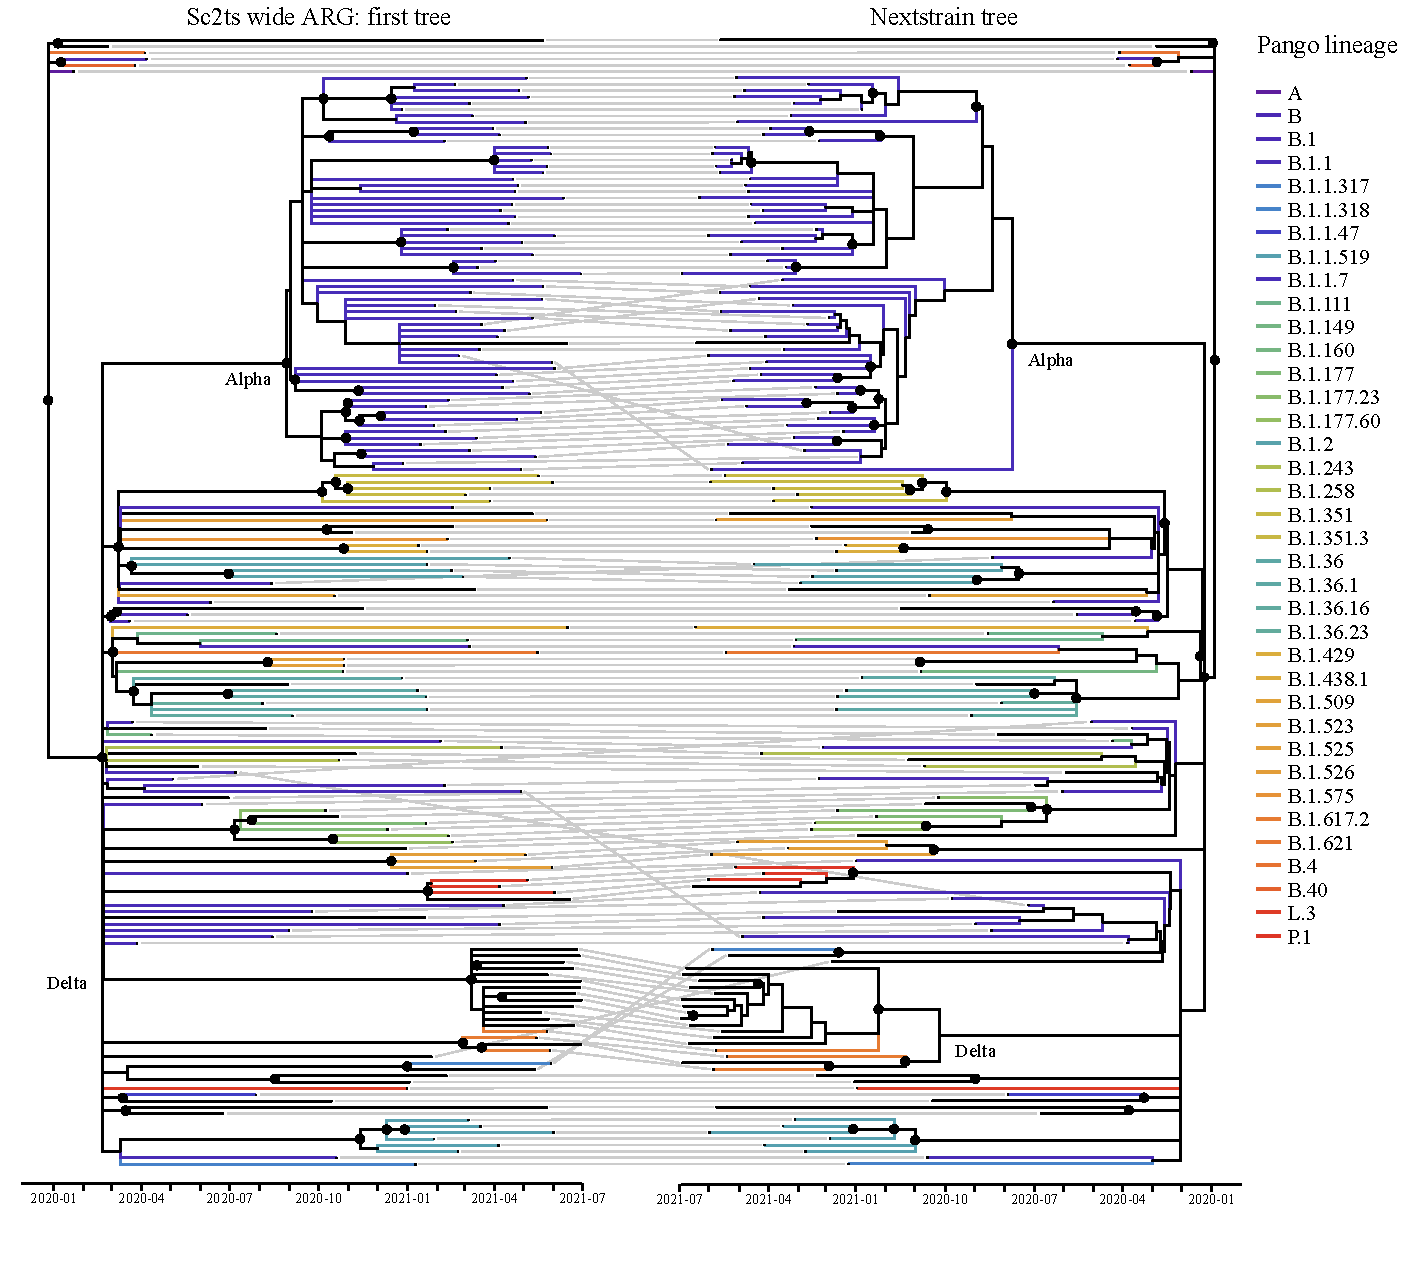
\includegraphics[width=\textwidth]{figures/cophylogeny_wide.pdf}
\caption{\label{fig:cophylogeny}
Tanglegram comparing the first local tree in the wide ARG (sampled to mid-2021)
and an ``all-time'' global NextStrain tree (sampled to January 21, 2023). The
trees were pruned down to the samples present in both the trees. Light grey
lines match the corresponding samples between the two trees; black circles
indicate identical sample partitions between the two trees. Terminal branches
are colour-coded according to the Pango lineage status assigned to the tip
samples; no Pango recombinants are shown, as none are shared between the trees.
The tanglegram was generated with the aid of the Neighbor-Net algorithm
\citep{Scornavacca2011-mg} implemented in Dendroscope version 3.8.5
\citep{Huson2012-ys}. See Figure~\ref{fig:cophylogeny_long} for the equivalent
cophylogeny for the Long ARG.}
\end{figure}

Figure~\ref{fig:cophylogeny} shows a co-phylogeny of the 88 samples shared
between the wide ARG and a GISAID global "all-time" tree from NextStrain
(downloaded on January 21, 2023). To reduce the ARG to a single tree, we show
the very first tree in the wide ARG; however, the five other trees in this
simplified ARG show near-identical patterns. Supplementary
Figure~\ref{fig:cophylogeny_long} shows the same comparison for the long ARG.
It is clear that the backbone topology of the sc2ts tree shows very close
agreement with the NextStrain tree. The sample genomes cluster by their
assigned Pango lineage status, and many variants and their descendents form
identical monophyletic clades in both the trees (e.g., the Alpha and Delta VoC
clades, labelled).

Figure~\ref{fig:cophylogeny} reveals some notable differences between the
trees. Firstly, the sc2ts tree is generally less well resolved (noticeably,
February to March, 2020). Secondly, there are non-identical sample partitions
near the tips (e.g., in the Alpha clade). These might have arisen because the
samples containing the mutations needed to resolve local topologies were
collected later than the cut-off date for the sc2ts ARG, but were for the
NextStrain tree. Finally, the branch lengths differ. For example, the branch
leading to the ancestral node of the Delta variant samples is much shorter in
the sc2ts tree than the equivalent NextStrain tree. It is possible that the
length of some of the branches was poorly calibrated, probably caused by overly
aggressive insertion of mutation-collapsing nodes and reversion-pushed nodes or
suboptimal sample attachment. Side-by-side comparison of sc2ts trees with trees
inferred using another method (e.g., UShER) should help to understand whether
branch length differences are due to poor calibration or methodological
differences.

Although the simplified backbone ARGs have few local trees, all of which show
essentially the same topologies, note that in the original ``un-simplified''
wide and long ARGs, there are 1,496 and 958 local trees respectively (Table 1).
Hence, while for a relatively small subset of the genealogy may be well
described by a single tree, the full dataset shows substantial variation in
phylogenetic relationships (i.e. ``phylogenetic incongruence'') across the
SARS-CoV-2 genome, much of which may be attributable to recombination. An ARG
representation is therefore essential to fully capture these reticulate
genealogical relationships.

\subsection{Mutational spectrum}
 In addition to recombination events, the ARGs record mutation events along the
SARS-CoV-2 phylogeny. \cite{Yi2021-sc} reconstructed a SARS-CoV-2 phylogeny of
over 350,000 genomes sampled globally from December 24, 2019, to January 12,
2021, and systematically catalogued all the mutations occurring along the
phylogeny. Notably, they described a mutational spectrum in which C-to-U and
G-to-U mutations occur more frequently than U-to-C and U-to-G mutations,
respectively.

\begin{figure} \centering
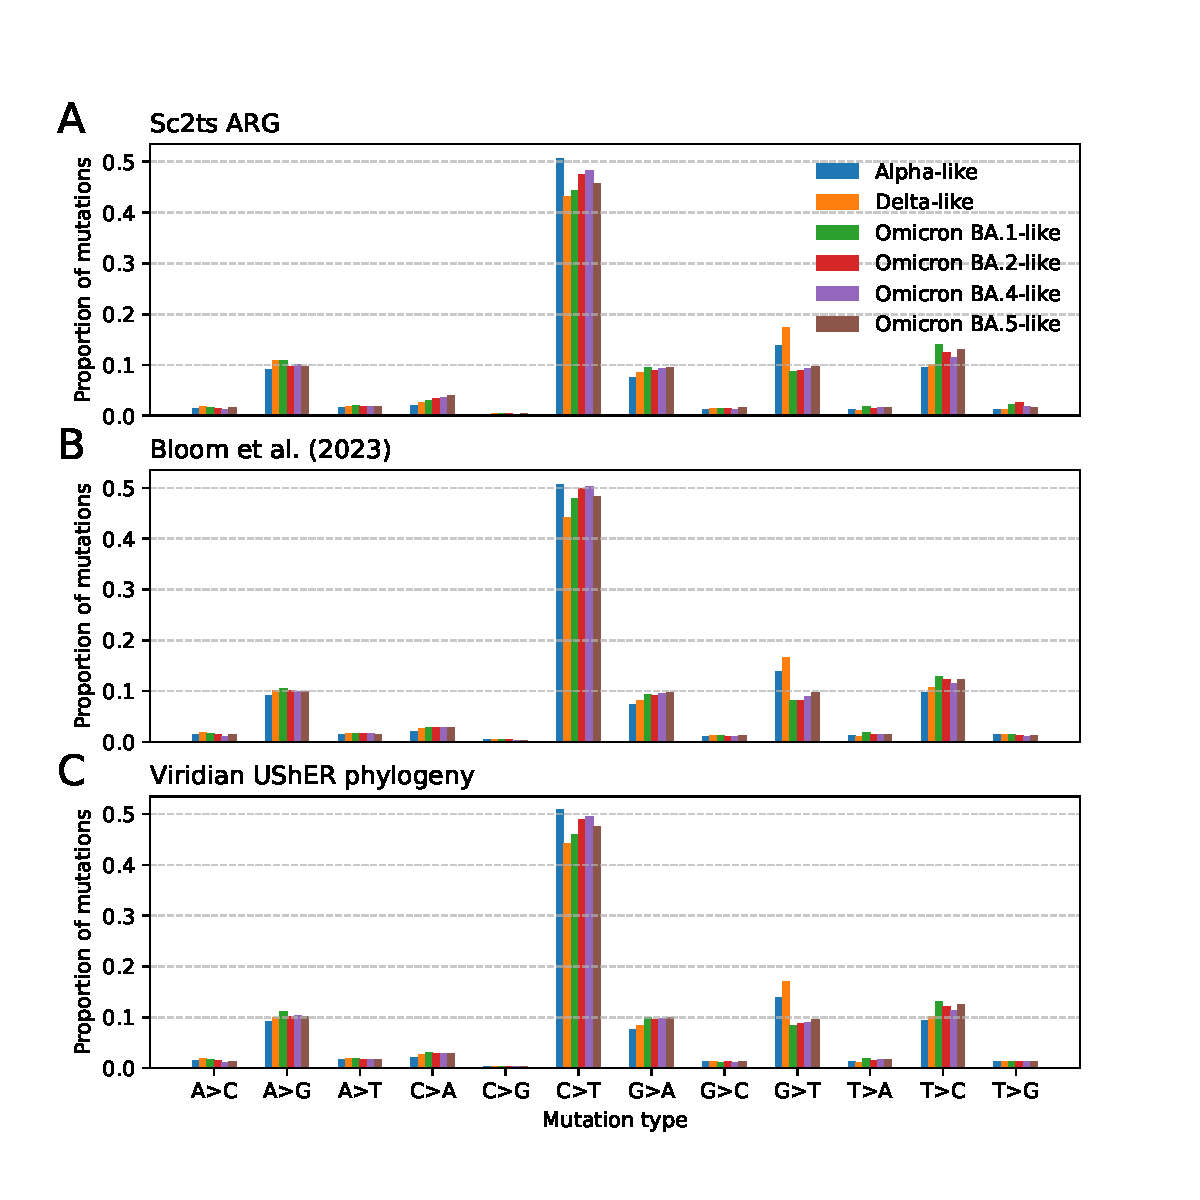
\includegraphics[width=0.4\textwidth]{figures/mutational_spectra.pdf}
\caption{\label{fig:mutational_spectra}
Mutational spectrum of SARS-CoV-2 in
the wide ARG (sampled to mid-2021) compared to \cite{Yi2021-sc}. Mutations are
categorised by type (i.e., ancestral state $>$ derived state). The percentages
of each mutation type from the wide ARG are represented by blue bars and the
percentages from Yi et al. by orange bars, with the darker colours representing
one direction (e.g., C$>$U) and the lighter colours the reverse (e.g., U$>$C).}
\end{figure}

For validation purposes, we compare the mutational spectrum from the wide ARG
with the mutational spectrum of \citet{Yi2021-sc}. We categorised all of the
single nucleotide mutations by type (defined by the ancestral state and derived
state), excluded mutations inherited by only a single sample (which are
enriched for sequencing errors and artefacts), and tallied them up by type.
Similarly, we took the data for single nucleotide mutations from
\url{https://github.com/ju-lab/SC2_evol_signature} \citep{Yi2021-sc}, excluded
mutations occurring along terminal branches, and tallied them up by type.
Figure~\ref{fig:mutational_spectra} shows that the mutational spectrum from the
wide ARG (based on 448,825 mutations) matches that reported by \citet[based on
92,344 mutations]{Yi2021-sc}. In both spectra, C-to-U mutations and G-to-U
mutations occur more frequently than U-to-C and U-to-G, respectively. Similar
results are obtained when including the mutations inherited by only a single
sample or those occurring on terminal branches (data not shown).

% If we do this, goes here
% \subsection{Mutations under selection}
% XX

\subsection{Early recombinants reported by Jackson et al. (2021)}
% - Early Recombinants from Jackson et al
%     Discuss results from Wide ARG in detail. Go into the details of the
% forward-backward HMM runs for each example. Be much more explicity about the
% single origin for the different groups (maybe give one of Ana's graphs for
% Group A (XA I think?)

By searching for samples combining genomic segments from Alpha (B.1.1.7) and
from the parental lineage B.1.1 based on a list of 22 Alpha-defining mutations,
\citet{Jackson2021-ik} reported 16 recombinant sequences among genomes sampled
in the United Kingdom up to March 7, 2021. The authors proposed that the
recombinants likely arose from eight independent recombination events
(categorised into groups A to D and four singletons).

% jk: this is the proposal from issue #33

\begin{table} \centering
\begin{tabular}{ll|clll}
\toprule
A Group (XA) & Jackson        &  21,256–21,613 & B.1.177/B.1.1.7 \\
             & \texttt{sc2ts} &  21,256--22,227 & B.1.177.18/B.1.1.7 \\
\midrule
B Group & Jackson        &  6,529--6,953 & B.1.36/B.1.1.7  \\
        & \texttt{sc2ts} &  6,529--6,954 & B.1.36/B.1.1.7  \\
\midrule
C Group & Jackson        &  25,997--27,441 &  B.1.1.7/B.1.221 \\
        & \texttt{sc2ts} &  25,997--27,972 &  B.1.1.7/B.1.221 \\
\midrule
D Group & Jackson        &  21,576--23,063 &  B.1.36.17/B.1.1.7 \\
        & \texttt{sc2ts} &  22,445--23,063 &  B.1.36.39/B.1.1.7 \\
\midrule
CAMC-CBA018 & Jackson        &  20,390--21,254 & B.1.177/B.1.1.7 \\
            & \texttt{sc2ts} &  16,177--21,255 & B.1.177/B.1.1.7 \\
\midrule
\end{tabular}
\caption{\label{tab:jackson}Comparison of recombination breakpoint intervals and parent lineages for a subset of the data reported by \cite{Jackson2021-ik}. [FIXME ADD MORE DETAIL] More detailed results are given in Table~\ref{tab:jackson_supplement}.}
\end{table}

In the wide ARG (sampled to mid-2021), all these sequences are descendants of
recombination nodes, except MILK-103C712, which was removed during
preprocessing (Table 2). Additionally, all except QEUH-1067DEF are HMM-consistent:
that is, the mirrored HMM runs (i.e. forward from 5’ to 3’ end versus backwards from 3’ to 5’ end)
identify the same set of originating mutations, have the same number of breakpoints, and have
equivalent (sequence-identical) parents from forward and backward runs.
Overall, we find excellent agreement between Jackson et al.’s
motif-based method and sc2ts in terms of (1) the Pango lineage of the parents
and (2) the breakpoint intervals (Table 2). In all cases, the two methods
proposed identical or very closely related parent lineages. The general mosaic
genome structure is concordant in all the cases, even CAMC-CB7AB3 where there
are two switches in the HMM copying paths (indicative of two breakpoints). The
breakpoint intervals estimated using the two methods overlap substantially in
all the cases (Table 2). Within each of the groups A to D, the constituent
sequences have identical breakpoint intervals, because they trace back to a
single recombination node in the wide ARG. This result is consistent with the
hypothesis that the sequences of the groups A to D emerged from four separate
recombination events~\cite{Jackson2021-ik}.

\subsection{Distribution of recombination breakpoint intervals}

% - Distribution of breakpoint intervals
%     Study the breakpoint intervals in the Wide ARG. Because we are interested
% in the intervals, we want to be sure that these are robustly reported by the
% HMM. Hence, we focus on those that have two parents in the mirrored and
% unmirrored HMM runs, the same set of mutations, and the left and right parents
% are consistently imputed for Pango lineage status.
%     We focus on the Wide ARG here because it covers (roughly?) the same time
% period as the RIPPLES analysis.

We explore recombination signals across the SARS-CoV-2 genome by inspecting the
breakpoint intervals of the filtered recombination nodes from the wide ARG
(sampled to mid-2021) in Figure~\ref{fig:breakpoint-distribution}. The length
of a breakpoint interval reflects uncertainty in the estimated location of a
breakpoint. On average, the length of the breakpoint intervals is 2,895 bases
(median, 1,670 bases; range, 1 to 23,666 bases). This broad distribution of
interval length indicates that the location of a breakpoint often could not be
precisely determined given the observed genetic variation.

\begin{figure}
\centering
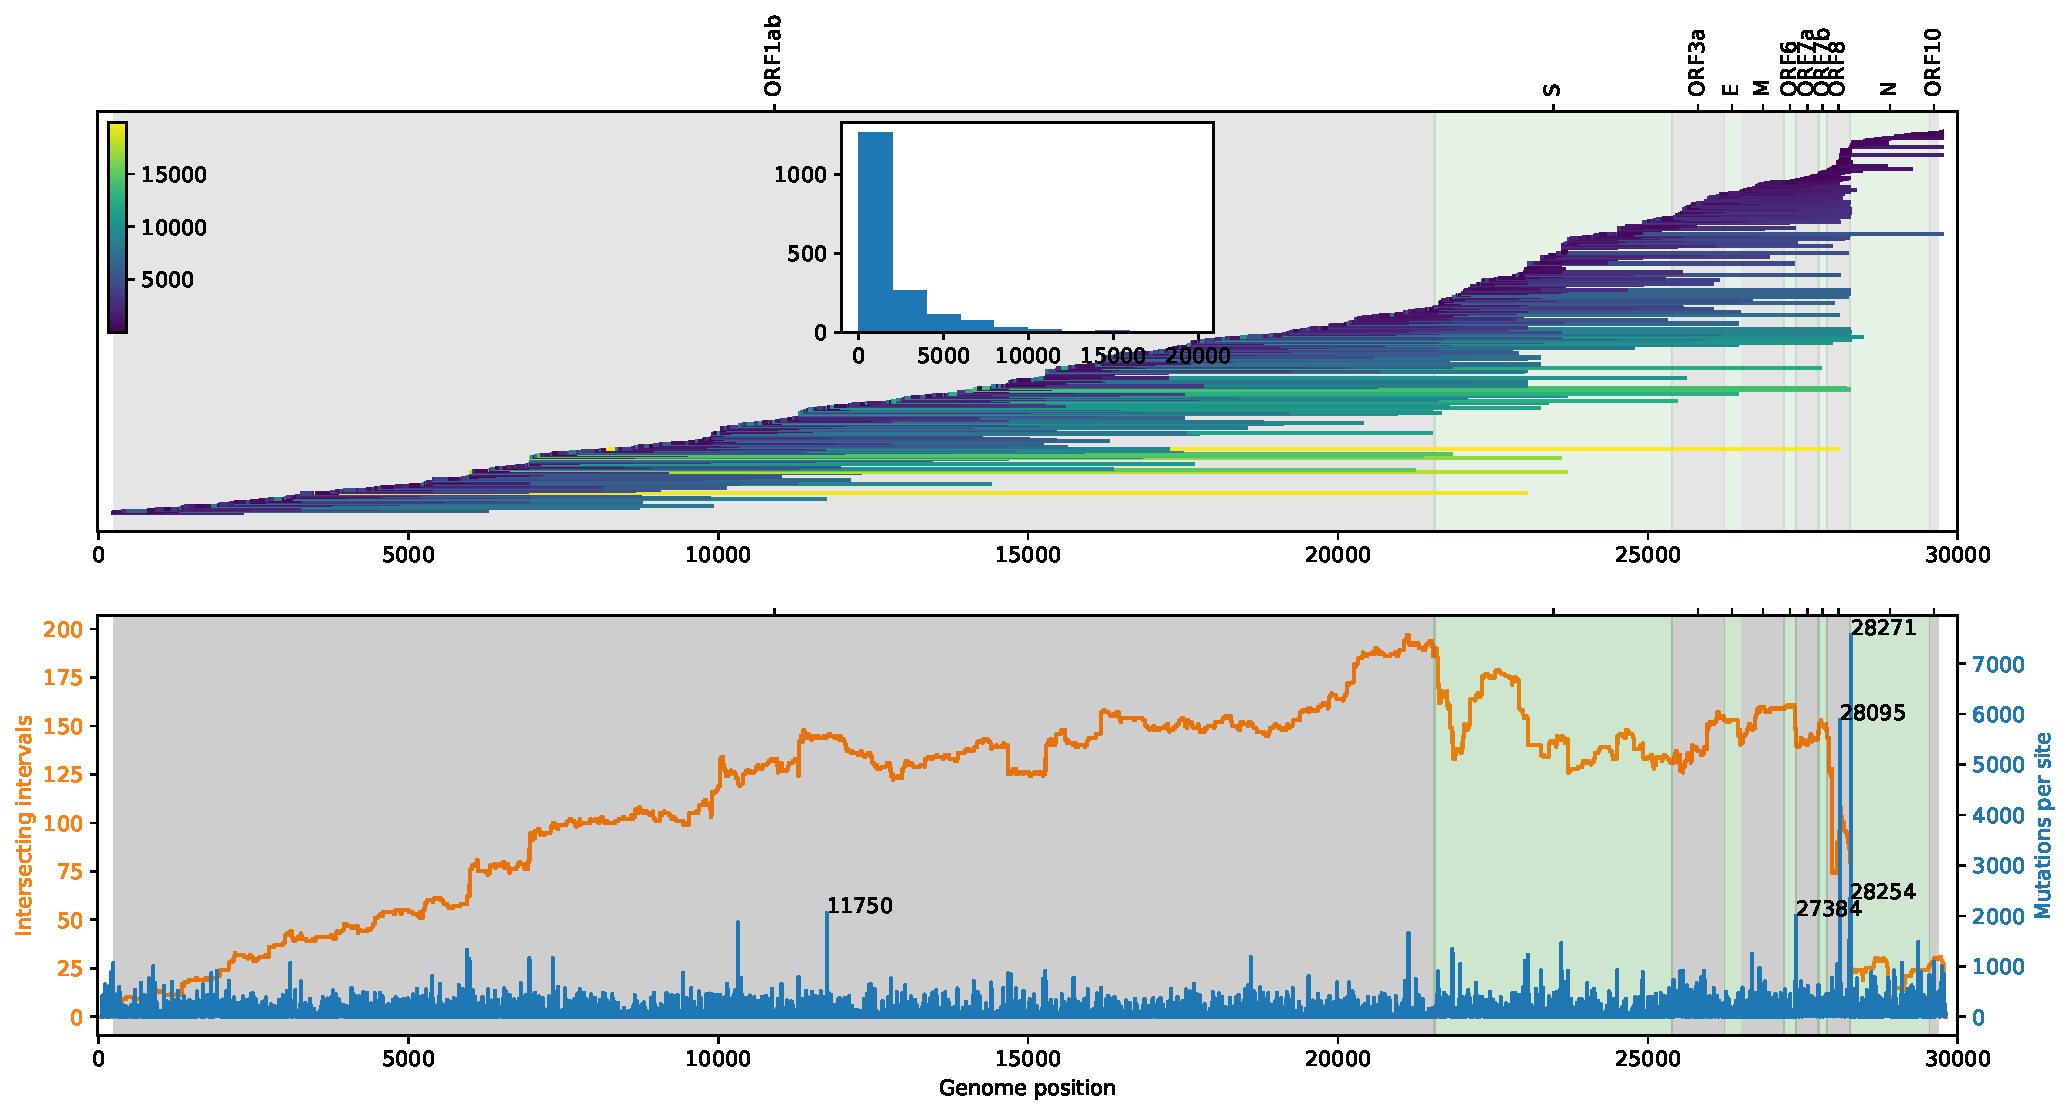
\includegraphics[width=\textwidth]{figures/recombination_intervals.pdf}
\caption{\label{fig:breakpoint-distribution}
Distribution of recombination breakpoints and mutations along the genome.}
\end{figure}

There is a preponderance of breakpoint intervals spanning the 3’ end of the
genome (Figure 4A), as noted previously by \cite{Turakhia2022-it}. Inspecting
more closely, we find an enrichment in the number of intersecting intervals in
the E gene, ORF8, ORF8-N intergenic region, and 3’ untranslated region (Figure
4B). Markedly, there is an abrupt drop in the number of intersecting intervals
in the N gene following the peak in ORF8 towards the 3’ end.

Next, we investigate the potential recombination signals alongside the number
of mutations across the genome (Figure 4C). Regions with a higher density of
mutations contain more genetic variation, increasing the power to detect
recombination events. The position 28,271 (located in the ORF8-N intergenic
region) has a particularly high number of mutations in the samples (Figure 5).
At this position, mutations (n = 7,572), insertions (n = 5,782), and deletions
(n = 1,605) appear to occur frequently. One possible explanation is that this
homopolymeric region is prone to sequencing errors, giving rise to an
artifactual recombination signal. At the upstream position 27,972, numerous
mutations also occur. This position has been reported to be hypermutable
\citep{Jungreis2021-dh}.

We further consider the breakpoint intervals within the context of
recombination breakpoint sequence motifs. It is hypothesised that certain
palindromic breakpoint sequences (specifically, CAGAC and CAGAT) promote
template switching during replication in SARS-CoV-2 via formation of
base-paired stem loops in the genome structure \citep{Gallaher2020-lb}. There
are 87 occurrences of these two breakpoint sequences in the Wuhan-Hu-1/2019
reference sequence (Supplementary Table 5). We observe that XX (XX\%) of the
breakpoint intervals of the HMM-consistent recombinants span at least one of
the breakpoint sequences.

\subsection{Divergence between recombinant parents}
% - Divergence between recombinant parents
%     We study the recombination events in the Long ARG in terms. A recombinant
% will not always have two parents, for reasons X, Y and Z. As a first
% approximation, we can assume that each breakpoint corresponds to a
% recombination event (although there are some exceptions). Here we have to get
% into all the hairy details about which sets of breakpoints we filter and don't
% filter.

\begin{figure} \centering
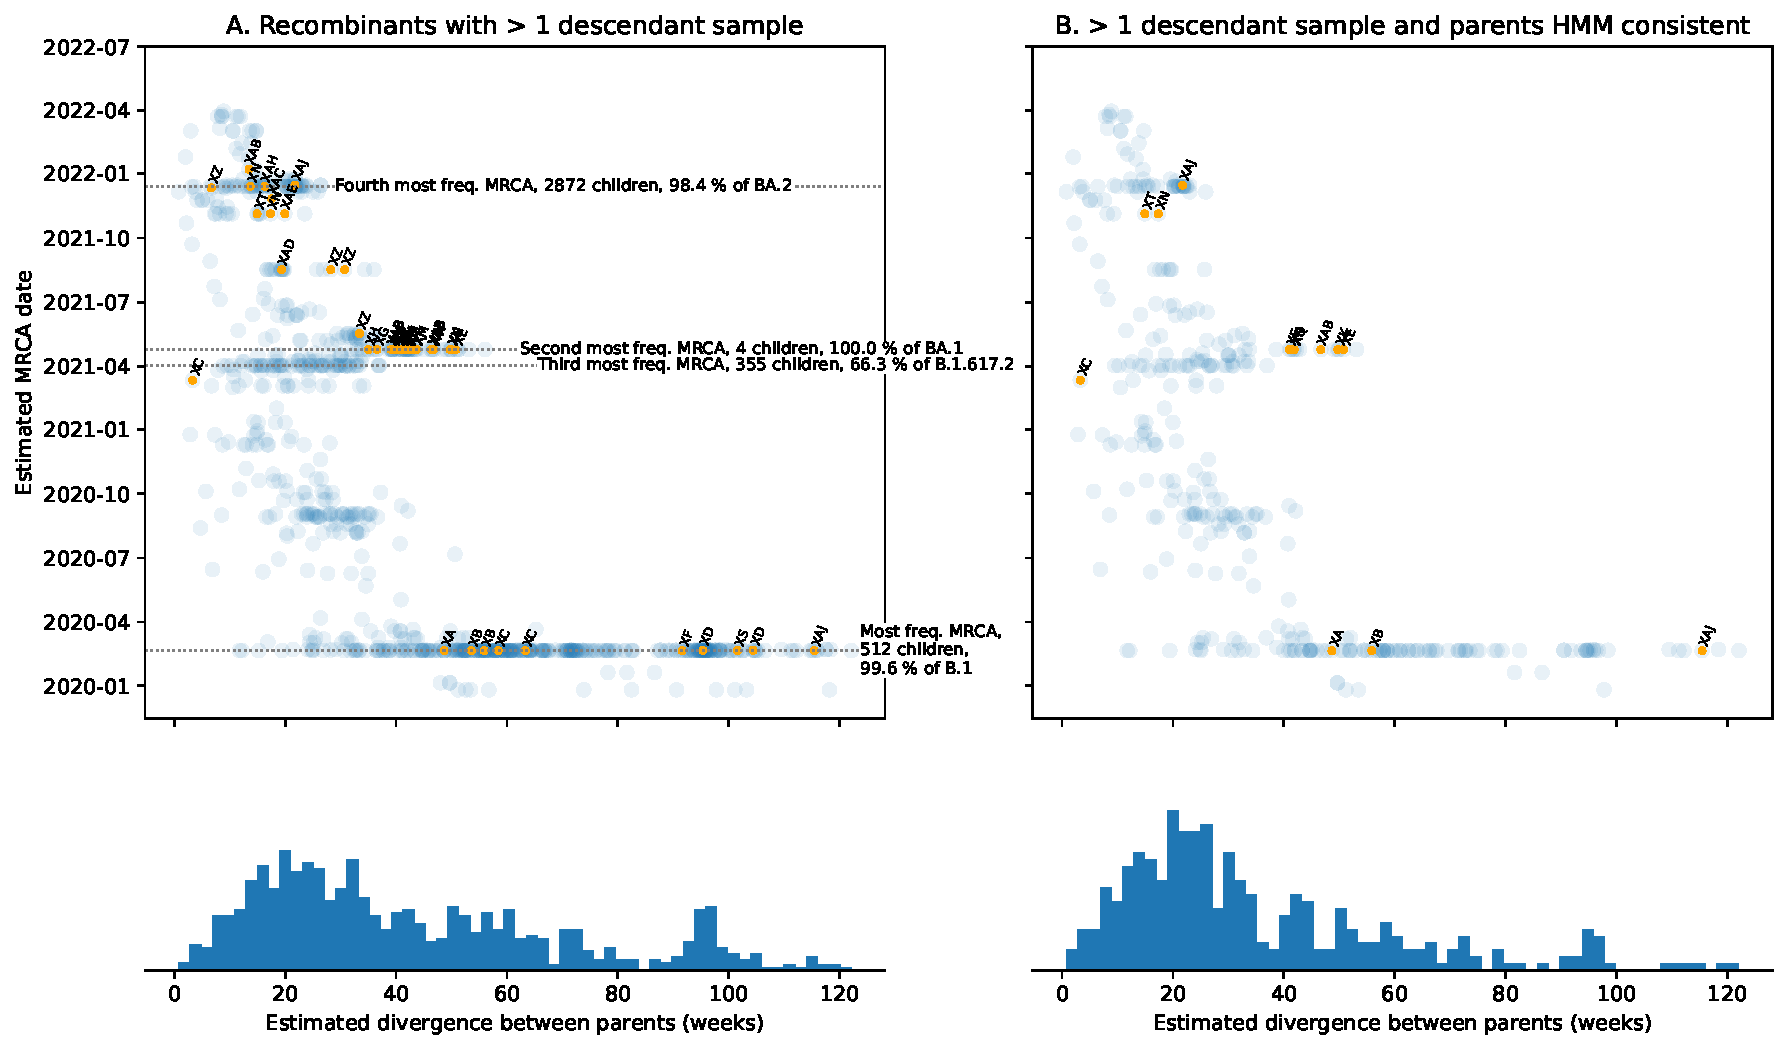
\includegraphics[width=\textwidth]{figures/recombination_node_mrcas.pdf}
\caption{\label{fig:recomb_mrcas}
Date of common ancestry between the parents either side of recombination
breakpoints, as a function of degree of parental divergence. MRCAs of parents
inferred to have produced a Pango designated recombinant (XA, XB, etc.) are
identified in orange (A) Data after removing singleton recombinants (XXX parent
pairs). Many recombinations involve parental strains that descend from the same
MRCA: dates for the four most frequently identified MRCA nodes are indicated by
horizontal dotted lines. These frequent MRCA nodes tend to be associated with
major waves and commonly have many immediate children (i.e. are large
polytomies, likely to indicate undersampled outbreaks) (B) Further filtered by
removing HMM inconsistent breakpoints (YYY parent pairs). Note that
Figure~\ref{fig:recomb_mrcas_voc_breakdown} shows the same data broken down by
parental VoC classification.}
\end{figure}

Both the wide and long ARGs contain a large number of recombination nodes (4123
and 2078 respectively; Supplementary Tables 1 and 2). Each of these nodes were
inferred as a result of matching a specific recombinant sample into the ARG.
However, ~63\% of recombination nodes are ancestral to only a single
recombinant sample; we exclude these "singleton recombinants" from subsequent
analyses as they may have arisen from sequencing of mixed samples (e.g., from
co-infection or contamination), and in any case, never result in onward
transmission.  This leaves 1522 and 763 recombination nodes in the wide and
long ARGs, respectively. In their analysis using RIPPLES,
\cite{Turakhia2022-it} detected 589 non-singleton recombinants.

We focus on the long ARG because compared to the wide ARG, it includes time
periods of increased rates of coinfection and recombination, and contains many
samples previously identified as the product of recombination (i.e. with a
Pango lineage designation starting with an "X"). Not only does the long ARG
capture all but one of the Pango designated recombinant lineages during this
time period (see the section below), but it also includes a large number of
non-Pango-identified recombinants. Many of these involve recombination between
relatively closely related lineages, as measured by the divergence time between
the recombination events and the most recent common ancestor (MRCA) shared by
the left and right parent at each breakpoint. As can be seen from
Figure~\ref{fig:recomb_mrcas}, this divergence time ranges from as little as
five or six days, to as much as several years in the case of recent
recombinants. This demonstrates that sc2ts can identify viral recombination
between very closely related lineages, providing a degree of resolution not
available with other recombination detection methods.

The histograms in Figure~\ref{fig:recomb_mrcas} show that
majority of newly identified recombinants arise from parents that diverged 10 to 30 weeks previously. However, there is also a peak of recombinants that diverged ~95 weeks prior to the event: these correspond to recombinants whose parental common ancestor traces to early 2020, including both Delta-Delta and Delta-Omicron recombinants (Supplementary Figure~\ref{fig:recomb_mrcas_voc_breakdown}). Note that each point in these plots represents a breakpoint, so that recombination events with more than one breakpoint (e.g. with 3 or more parents, which comprise X \% of the recombination events) are represented by several plotted points.

As a check on the reliability of these identified recombination events,
Figure~\ref{fig:recomb_mrcas}B  plots only those breakpoints which are
HMM-consistent. This reduces both the number of recombination nodes /
breakpoints from 1522 / B to C / D in the wide ARG and from 763 / 806 to 459 in
the long ARG (Supplementary Tables 1 and 2).

The date of common ancestry for the two parents of recombinant lineages is
concentrated in several banded rows in Figure~\ref{fig:recomb_mrcas}. These are
largely due to a small handful of MRCAs which are shared between a large number
of recombination events; the top four are indicated by dotted lines in the
figure. These shared MRCAs are near the root of large expansions of certain
lineages (B.1: original variant;  B.1.617.2: Delta, BA.1: first Omicron wave;
and BA.2: second Omicron wave), as evidenced by the number of samples with that
Pango designation that trace back to these ancestral nodes (listed as
percentages on the plot). The specific MRCA nodes to which many recombinants
trace frequently represent very large polytomies in the tree (at the extreme,
2,872 immediate children). This is likely to indicate a rapid and under-sampled
expansion of a clade in the SARS-CoV-2 genealogy.

Finally, it is clear from Supplementary Figure 4 that of the recombinant
parents that fall into the Alpha, Delta, and Omicron VoC classes, the majority
are within-Delta and within-Omicron recombinants, and that Omicron followed by
Delta, are the variants associated with the most recombination. This may
reflect either sampling intensity, the prevalence of cases (which increases the
chance of coinfection and recombination), or possibly heterogeneity in
recombination probabilities among lineages.

\subsection{Recombinant Pango lineages}

In this section we focus on the detailed genealogy of samples that have been
previously identified as recombinants, i.e. given a Pango designation that
starts with an ``X''. Since the wide ARG is restricted to data collected prior
to mid-2021, it contains samples from only three Pango-designated recombinant
lineages: XA, XB, and XC. To investigate the diversity of genealogies
associated with recombinants, we therefore devote more analysis to patterns in
the long ARG. As in previous sections, we exclude singleton recombinants where
possible.

\subsubsection{Wide ARG}
[Quick overview of the wide ARG.]
In the wide ARG, 44
samples are designated as XA by both Nextclade and GISAID, 237 are designated
as XB by Nextclade (231 by GISAID), and 6 as XC by Nextclade (none by GISAID).
After removing singleton recombinants, XA numbers remain unchanged, but XB is
reduced to 235 (229) and XC to 4 (0). We correctly identify that all samples
designated as XB by any method have one or more recombination nodes in their
ancestry.

The simplest Pango recombinant genealogy is XA: all XA samples trace back to a
unique originating recombination node. This is the product of a recombination
between a B.1.177.18 sample (specifically the strain Wales/ALDP-115BF41/2021,
EPI\_ISL: 1012804) which contributed the majority of the genome from the start
to a maximum position of 22227bp, and an unknown (inserted) node with imputed
Pango lineage B.1.1.7, which contributed the remaining right hand portion. The
recombination node has five immediate children: four sample leaves (EPI\_ISLs:
989697, 1019487, 1104468 and 1122630) and a UPGMA-inserted node which is the
ancestor of all other XA samples in the dataset.

For XB, all samples trace back to a originating node which is the product of a
recombination between a B.1 sample (specifically the strain
England/CAMB-7B47D/2020, EPI\_ISL\_433960, which contributed the majority of
the genome from the start up to a maximum position of 23604bp), and two other
UPGMA nodes with imputed Pango lineages B.1.627 (up to a maximum position of
27389bp) and B.1.36.8 (the remaining fragment of the genome). As described
later, in the long ARG the equivalent recombination node has only 2 parents,
with no involvement of  B.1.36.8, and it is possible that the third parent in
the wide ARG is artifactual. Additional complications arise because additional
non-X-designated samples such as B.1.634 also descend from this recombination
(also true in the long ARG, see below), and there are also a small number of
further recombination nodes nested within the XB ``clade''. However, all but
one of these nested recombinations are ancestral to only a negligible fractions
of the designated XB samples. The exception accounts for about 17\% of the
designated XB nodes, and involves a recombination between descendants of the
originating XB recombination. More specifically strain
USA/TX-HMH-MCoV-43092/2021 (EPI\_ISL 2224652) is inferred to be a recombination
between an XB grandparent and its XB grandchild. This could well be
artifactual.

For XC, the wide ARG identifies more than one originating recombination node
(see "multiple origins" below). However, as none of the samples designated as
XC by Nextclade are designated as XC by GISAID, these patterns could be due to
mistaken labelling, hence we do not examine XC further.

\subsubsection{Long ARG}
[high level summary of the pango recombinant lineages
and samples in the Long ARG]
The long ARG (subsampled to mid-2022) contains 33
Nextclade-designated Pango recombinant lineages (XA to XAK; Supplementary Table
XXX) comprising 749 samples (711 when singleton recombinants are removed). If
the GISAID designations are used, 38 Pango lineages exist in the long ARG,
comprising only 515 samples. In the analyses below, we mainly focus on the
larger number of Nextclade designated samples.

Of the 749 Nextclade recombinant samples, all but 2 are inferred to descend
from a recombination node. These two samples are designated XP, and a likely
explanation for their not have an inferred recombinant origin in the long ARG
is that the characteristic multibase deletion for XP
(\url{https://github.com/cov-lineages/pango-designation/issues/481}) is masked
during preprocessing. An improved masking pipeline is an important avenue for
future development (see the Discussion).

38 of the remaining X designated samples are singleton recombinants, descending
from recombination nodes that are ancestral only to that sample (10 are XZ; 6
are XE;  3 each from XN and XK; 2 each from XC, XS, XV, XQ and XAB; and 1
sample from each of XB, XM, XJ, XAF, XAH and XAJ). Such samples are likely to
be enriched for sequencing errors and lineage designation artefacts, and so we
exclude them from further analysis in this section.

The most recent recombination node for 79 samples (XN: 53, XZ: 16, XAJ: 6, XE:
1, XAD: 1, XAH: 1, XAK: 1) is the same. This node is ancestral to more than
127K samples, and is likely to be a spuriously inferred recombination event.
Understanding the origin of this and other similar nodes, is an important
direction for future work (see Discussion). For simplicity, we exclude these
samples from further analyses in this section.

The remaining remaining 630 Pango X designated sequences trace back to 50
different recombination nodes. We examine the inferred inheritance structure in
the following subsections.

% The sequences of 28 Pango recombinants trace back
% to some recombinant node(s); however, the sequences of the five Pango
% % jk: really? I thought it was just XP that wasn't inferred to be a
% % recombinant.
% recombinants XP, XU, XAA, XAG, and XAK do not.
% A likely explanation for the XP
% recombinant sequences not having a recombinant origin in the long ARG is that
% its characteristic multibase deletion
% (\url{https://github.com/cov-lineages/pango-designation/issues/481}) was masked
% during preprocessing and therefore was not incorporated into the HMM.
% % Eh?
% Upon tracing the origin of XAG through the ARG, XAG might have been caused by
% incorrect imputation of its parent nodes(?). XAK likely does not appear to have
% a recombinant origin because of random subsampling, but it may with a more
% complete tree.

% [FIXME this isn't quite right - not all the sequences for a given pango
% lineage trace back to the same recombination event, so won't have the same
% intervals.]
% The mosaic genome structure of all the 32 Pango recombinant lineages is concordant with
% the structure determined by the Pango Lineage Designation Committee
% (Supplementary Table 3). For example, the genome of XD (also known as
% ``Deltacron'') is inferred to consist of B.1.617.2 (Delta) on the 5’ end, BA.1.17
% (Omicron) in the middle, and B.1.617.2 (Delta) on the 3’ end.

% For the long ARG, we examine the lineages in increasing complexity of the
% inferred evolutionary relationships between samples assigned to Pango
% X lineages.

% - Recombinant Pango lineages
%     How well do we recover recombinant Pango lineages? Work through the
% examples in increasing compexity, using headings to split things up if
% necessary. (i.e., Single origin, Multiple origin, Interellated lineages). We'd
% need to be clear about what these terms mean, of course. We could include
% lineage graphs for all of these examples?

% OLD TEXT

% The sequences of 14 Pango recombinants trace back to a single recombination
% node. The sequences of the remaining 18 Pango recombinants trace back to
% multiple recombination nodes, however. This may be a result of undersampling in
% the long ARG, which was built by randomly subsampling at most 1,000 sequences
% from each daily batch. Having extra recombination nodes in the long ARG
% appeared to be a more parsimonious explanation for the 19 Pango recombinants
% than having a single recombination node with many immediately ancestral
% mutations (including recurrent mutations and reversions), despite that the
% recombinants may indeed trace to a single origin.

\subsubsection{Single origin}
We would usually assume that all sequences
assigned to a given Pango X lineage are descendants of a single recombinant
sequence, arising as a result of a mixed infection followed by onward
transmission. Thus, we would also expect our ARG to reflect this evolutionary
history, where we have a all the samples assigned to this recombinant lineage
tracing back to a single recombination node, representing this original
recombination event.

\begin{table}
% \begin{footnotesize}
\begin{tabular}{lllrl}
\toprule
{} &              parent\_lineages &          pango\_parents &   n &
descendant\_lineages \\
lineage &                              &                        &     &
\\
\midrule
XA      &        [B.1.177.18, B.1.1.7] &     [B.1.1.7, B.1.177] &   5 & XA: 5 \\
XAA     &               [BA.1, BA.2.9] &         [BA.1*, BA.2*] &   8 &
    XAB: 39, XAG: 17, XAA: 8 \\
    &&&&   XAA: 8, XQ: 2, XU: ... \\
XAC     &          [BA.2.3, BA.1.17.2] &  [BA.2*, BA.1*, BA.2*] &  27 & XAC: 27 \\
XAE     &                 [BA.2, BA.1] &         [BA.2*, BA.1*] &   9 & XAE: 9 \\
XAG     &               [BA.1, BA.2.9] &         [BA.1*, BA.2*] &  17 &
    XAB: 39, XAG: 17, XAA: 8 \\
    &&&&   XAA: 8, XQ: 2, XU: ... \\
XF      &                 [AY.4, BA.1] &    [B.1.617.2*, BA.1*] &   2 & XF: 2 \\
XG      &              [BA.1.17, BA.2] &         [BA.1*, BA.2*] &  32 & XG: 32, XAB: 1 \\
XH      &            [BA.1.20, BA.2.9] &         [BA.1*, BA.2*] &  11 &
    XAF: 34, XH: 11 \\
&&&& B.1.1.529: 3, XE: 3,... \\
XK      &             [BA.1.1.1, BA.2] &         [BA.1*, BA.2*] &   6 & XK: 3 \\
XL      &            [BA.1.17.2, BA.2] &         [BA.1*, BA.2*] &  10 &
    XL: 10, XAB: 1, XU: 1, \\
    &&&& XQ: 1 \\
XR      &               [BA.1.1, BA.2] &       [BA.1.1*, BA.2*] &   8 &
    XQ: 9, XR: 8, XAB: 2\\
XS      &              [AY.36, BA.1.1] &  [B.1.617.2*, BA.1.1*] &   6 & XS: 4\\
XT      &       [BA.2.23, Unknown (R)] &         [BA.2*, BA.1*] &   1 &
    BA.2: 1, BA.1: 1, BA.1.9: 1, \\
    &&&& BA.2.23:... \\
XV      &  [BA.1.1, BA.2, Unknown (R)] &         [BA.1*, BA.2*] &   3 & BA.2: 8, XV: 1 \\
XW      &            [BA.1.1.15, BA.2] &         [BA.1*, BA.2*] &  11 & XW: 11, XN: 2 \\
XY      &               [BA.1.1, BA.2] &         [BA.1*, BA.2*] &   6 & XY: 6, XAF: 1 \\
\bottomrule
\end{tabular}
\caption{\label{tab:pango-single-origin}
Table summarising the status of the Pango X-lineages in the Long ARG thare inferred to have a single recombinant origin based on the NextClade Pango lineage assignments. Imputed parent lineages are shown from the ARG and also to parent lineages as defined by the official Pango designation alias key. FIXME: if we like this table then we can reformat it so that lists at the end are spread over multiple lines rather than using Python dict notation }
\end{table}

\begin{figure}
\begin{tabularx}{\textwidth}{c}

% \end{footnotesize}
% \\

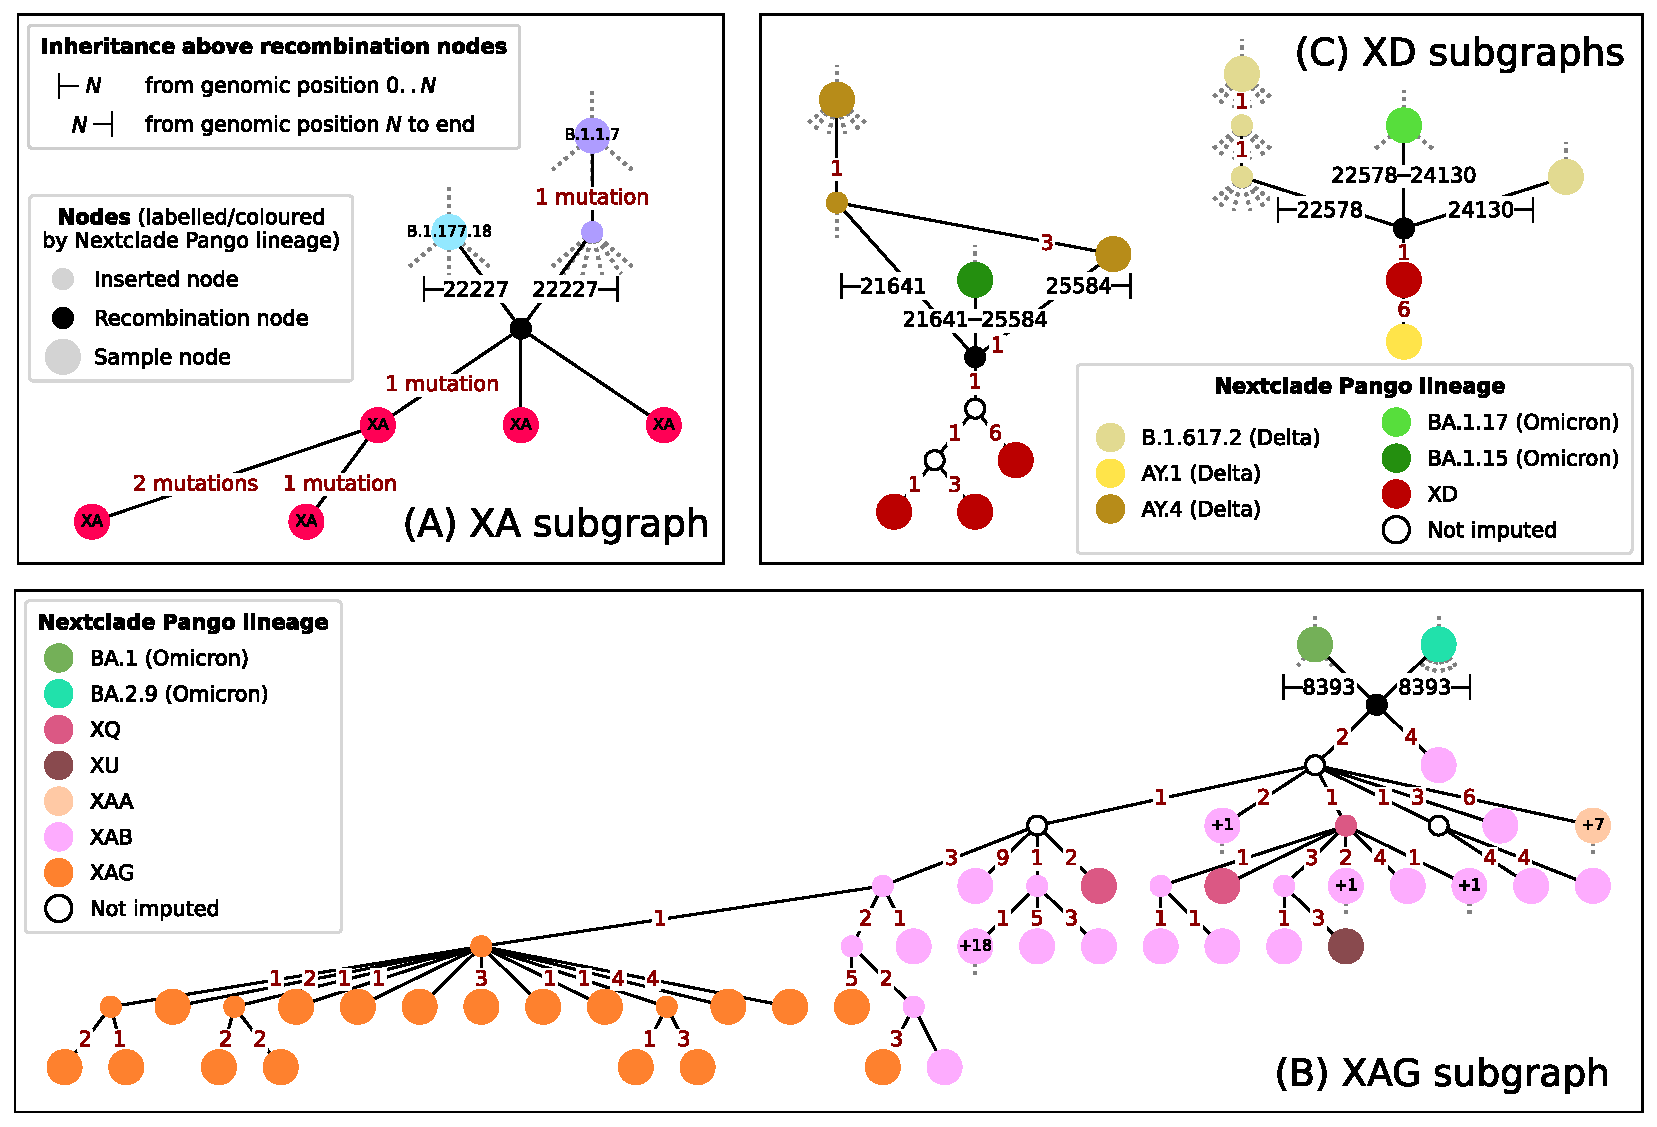
\includegraphics[width=\textwidth]{figures/Pango_XA_XAG_XD_nxcld_tight_graph.pdf}
% }
\end{tabularx} \caption{\label{fig:pango-simple-origin-graph} Simple origin
Nextclade Pango X lineages. (A) Subgraph for XA in the long ARG: all five samples designated
as XA by Nextclade, together with their ancestral lineages, are shown outwards to the nearest
sampled viral genome; dotted lines show ARG continuation. Nodes are coloured by Nextclade
Pango designation; smaller symbols are non-sample nodes inserted by sc2ts, with
imputed Pango status. (B) Equivalent plot for the 17 XAG samples in the long ARG
(C) Equivalent plot for both origination events for the four XD samples in the long ARG.
} \end{figure}

In Figure~\ref{fig:pango-simple-origin-graph}A we illustrate the case of XA. We construct a small subgraph of the long ARG, tracing routes from Nextclade-identified XA samples to the closest other sample strains in our dataset. Where a route passes upwards through a recombination node, we only show the continuing parental lineages to the most recent sample ancestors, rather than descending the ARG downward to cousins of the recombinant parents. Dotted lines show where this subgraph links to other nodes within the ARG. It is clear from the subgraph that all the XA samples trace to a single originating recombination node.

Table~\ref{tab:pango-single-origin} summarises the sequences of all 16 of the
Pango recombinant lineages that trace back to a single recombination node in
the long ARG. [FIXME UPDATE THESE] We can see that XA, XAC, XAE, and XF form
monophyletic clades, in which all of the samples given that Pango designation
descend from a single recombination node.

[Discuss remaining]

There is generally good agreement on the imputed parental lineages from the ARG
and the official Pango designations. [Discuss more]

[Discuss panel B where XAG shares a common recombinant origin with samples from
several other X lineages]

Figure~\ref{fig:pango-simple-origin-graph}B shows a case of another
Pango lineage, XAG, whose Nextclade-designated samples also trace to a
single originating recombination. This is a more intricate example, as the same origin
is also shared with all samples designated XAA, and some, but not all, of the
samples identified as XAB, XQ, and XU by Nextclade. Note, however, that if the GISAID
designations are used, many of the samples marked here as XAB are reclassified
as BA.2, and XAG becomes fully monophyletic (supplementary figure
\ref{fig:pango_XAG_gisaid_graph}, which also gives identifying labels to the
sample nodes, convertable to EPI\_ISL identifiers using
Supplementary table XXX )

\subsubsection{Multiple origins} The ARG inference has no pre-defined knowledge
of Pango X lineage assignments, and there is therefore no particular
requirement that all the samples assigned to a given lineage must trace back to
a single recombination event. In this section we examine the Pango X lineage
samples that are inferred to have multiple recombinant origins (i.e., trace
back to different recombination nodes in the ARG), but still form monophyletic
clades % is this the right term? descending from these nodes .

% \begin{frame}
% \begin{block}{Multiple origin Pango X lineages}
% \begin{itemize}
% \item For the remaining 18, the story is more complicated.
% \item XJ, XU and XV each have 3 samples and 3 recombinants
% \item One recombinant shared among 5 lineages (XAA, XAB, XAG, XQ, XU)
% \item XE has 170 samples and 12 recombinants; some are very similar
% (Official: BA.1* \& BA.2, 10448--11287):
% \\
% \vspace{1em}
% \begin{tabular}{llll}
% \toprule
% Left parent & Right parent & \multicolumn{2}{l}{Breakpoint interval}\\
% \midrule
% BA.1.15 & BA.2  &9867  &10198\\
% BA.1.15 & BA.2  &9867  &10198\\
% BA.1.1  &BA.2  &10451  &11537\\
% BA.1.1.5 & BA.2 &10448 & 11537\\
% BA.1.15 & BA.2  &10448  &12880\\
% BA.1.17 & BA.2  &10448 & 11537\\
% BA.1  &BA.2.9  &10448 & 11537\\
% BA.1  &BA.2  &12764  &13195\\
% \bottomrule
% \end{tabular}
% % BA.3  &BA.1.17  &22674  &22674\\
% % BA.1.1.15 Recombinant 10448 11537
% % BA.1.1 Recombinant 10030 10447
% % Recombinant BA.2 17411 19955
% \end{itemize}
% \end{block}
% \end{frame}


\begin{figure}

\begin{tabular}{llll}
\toprule
Left parent & Right parent & \multicolumn{2}{l}{Breakpoint interval}\\
\midrule
BA.1.15 & BA.2  &9867  &10198\\
BA.1.15 & BA.2  &9867  &10198\\
BA.1.1  &BA.2  &10451  &11537\\
BA.1.1.5 & BA.2 &10448 & 11537\\
BA.1.15 & BA.2  &10448  &12880\\
BA.1.17 & BA.2  &10448 & 11537\\
BA.1  &BA.2.9  &10448 & 11537\\
BA.1  &BA.2  &12764  &13195\\
\bottomrule
\end{tabular}
% BA.3  &BA.1.17  &22674  &22674\\
% BA.1.1.15 Recombinant 10448 11537
% BA.1.1 Recombinant 10030 10447
% Recombinant BA.2 17411 19955
\caption{\label{tab:multiple_origins_table}
details of inferred
breakpoints for different recombination events inferred for XE samples (170
samples and 12 inferred recombination nodes; some are very similar (Official:
BA.1* \& BA.2, 10448–11287)}
\end{figure}

Figure~\ref{fig:pango-simple-origin-graph}C shows a simple example, consisting of
the 4 samples labelled XD by Nextclade in the long ARG. The left hand subgraph
(the origin of three XD samples) has an earliest
sample with EPI\_ISL: 11222324 (dated 2022-02-26), while the right hand
subgraph has a single sample with EPI\_ISL 8514045 (dated 2021-12-30). These
two samples differ by 35 mutations; considering this, and the time between the samples,
it does seem possible that they represent true independent origins of XD.
Supplementary Figure~\ref{fig:pango_XD_gisaid_graph} shows the same subgraphs
with sample identifiers and coloured by GISAID Pango labels (however, no
samples are designated by GISAID as XD in the long ARG).

Table \ref{tab:multiple_origins_table} summarises other Pango recombinants which
we infer to have multiple origins. [TODO: needs more detail]


\subsubsection{Complex origins} 
\begin{figure} \centering
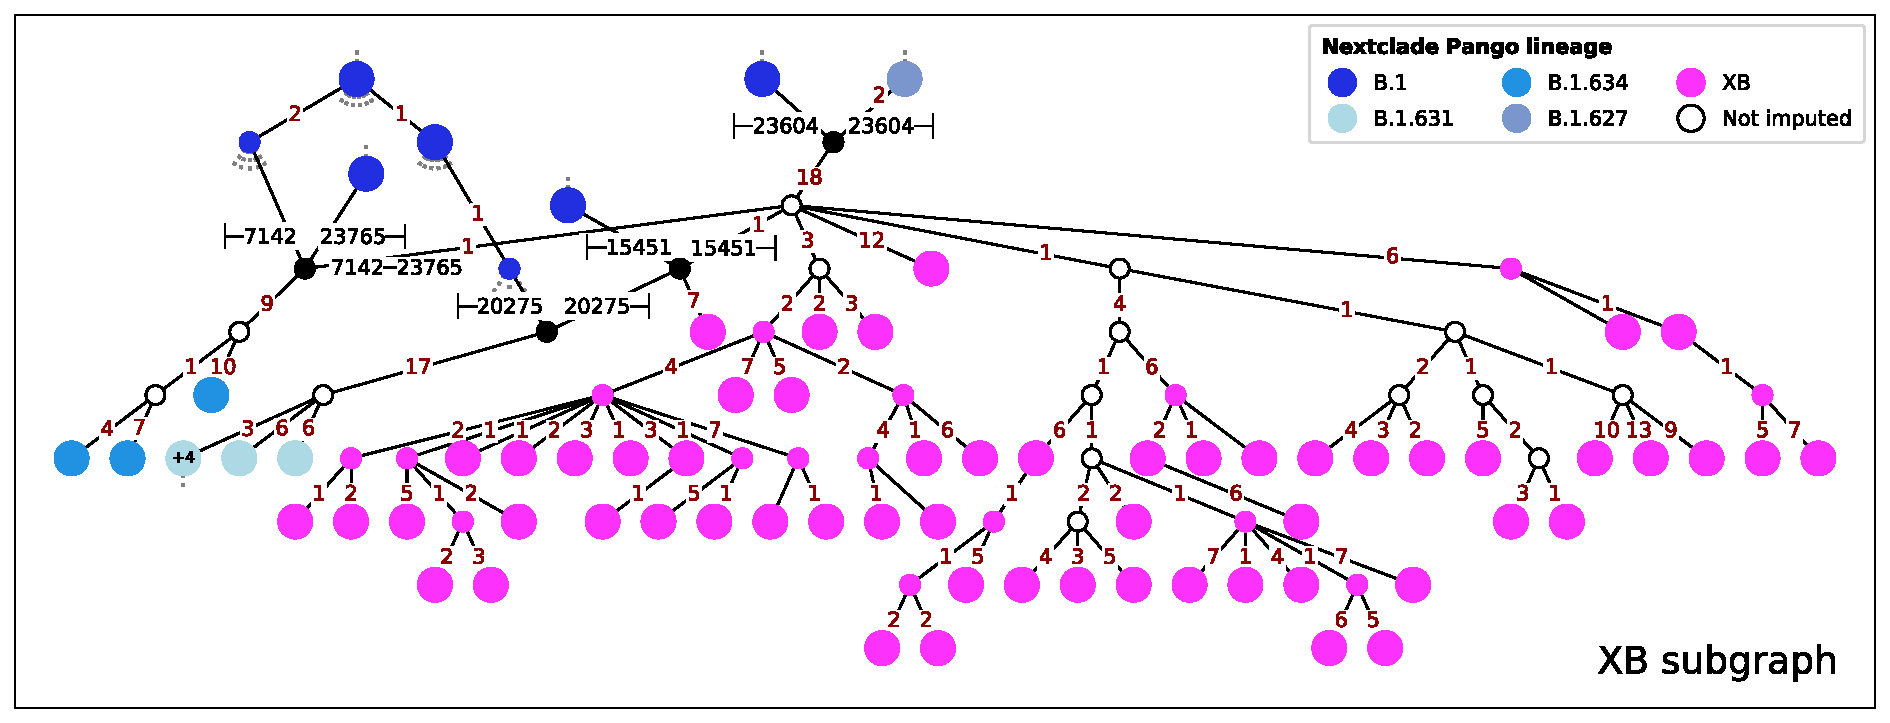
\includegraphics[width=\textwidth]{figures/Pango_XB_nxcld_tight_graph.pdf}
\caption{\label{fig:complex_origins_graph}  A Pango lineage subgraph showing
complex origins of the recombinant lineage XB. All XB samples in the long ARG
trace to a single recombination node (top centre), but three further recombinations
also descend from this node, with many samples descending from these nested
recombinations not being identified as XB, but instead assigned by Nextclade to
various pre-Alpha lineages.}
\end{figure}

As well as cases where single recombination events explain an X lineage,
such as the examples in Figure~\ref{fig:pango-simple-origin-graph}, many of the
Pango X lineages involve more complex origins,
in which additional recombination events are nested inside the earliest shared
recombination. Frequently, the descendants of the original recombination
also include samples which have not been previously identified as recombinants.
An example is XB in the long ARG,
plotted in Figure~\ref{fig:complex_origins_graph}. Here, a recombination
between a B.1 sample and B.1.627 sample leads both to the XB samples and to a
``hairball'' of further recombination nodes whose descendants have not been
identified as recombinants by Nextclade (blue nodes, ``pre-Alpha'' VoC). However,
in this subgraph, there is only a single sample, identified as XB by Nextclade,
which is descended from these nested recombination events; moreover, this
sample is not identified as XB by GISAID (Supplementary
Figure~\ref{fig:pango_XB_gisaid_graph}). We suggest that investigating cases of
complex origins, and identifying which (if any) of the nested, further
recombination events may be artifactual, is an important area of future
research.

% JK: removing this for now

% \subsection{Novel recombinants}
% Next, we examine recombination nodes in the
% long ARG (sampled to mid-2022) that represent previously unnamed putative
% recombinant sequences, which do not have a Pango recombinant designation. For
% this proof-of-concept study, we have arbitrarily picked 12 recombination nodes
% that seem plausible (Supplementary Table 4). All these nodes involve Omicron
% subvariants (BA.1, BA.2, BA.4, and BA.5). These recombination nodes (1) were
% inserted into the long ARG on or after January 8, 2022; (2) have at least 10
% descendent samples; and (3) have no mutational differences (including immediate
% reversions) from their parent nodes.

% TODO: Node  740761 (USA/NC-CDC-LC0668306/2022) is a sister clade proposed1006
% in the UShER public phylogeny. Node 628656 (Scotland/QEUH-37794BB/2022) is a
% sister clade of XAC, and annotated as ``miscBA2BA1PostSpike''.

\section{Discussion}
The COVID-19 pandemic continues to be a global emergency,
with persistent high levels of infection. This high prevalence has allowed the
proliferation of many variants, with more than 600 Pango-designated lineages
circulating globally in the last three months (January to March, 2023;
https://gisaid.org/; access on March 27, 2023). High prevalence also brings a
higher risk of coinfection, increasing opportunities for new phenotypically
distinct recombinants to emerge and spread.

In this proof-of-concept study, we demonstrate the feasibility of
reconstructing a large ARG from over one million SARS-CoV-2 genomes, a feat
that is simply not possible using other available ARG inference methods
\citep{Rasmussen2014-el,Ignatieva2021-rg, Speidel2019-yh}. We have accomplished
this feat by building on top of recent advances in storing and processing large
ARGs (tskit) and inferring genealogical relationships efficiently at scale
(tsinfer). The highly compact representation of the ARGs as succinct tree
sequences, coupled with vectorised computing technologies, enables the large
SARS-CoV-2 ARGs to be loaded in less than one second in a Jupyter notebook and
allows for each SARS-CoV-2 genome to be stored in less than eleven bytes of
data. We believe that further development of the sc2ts methodology and software
can create a powerful tool (1) to efficiently detect emerging or previously
overlooked recombinants in SARS-CoV-2; (2) to jointly model the mutational and
recombinational processes shaping global SARS-CoV-2 genomic diversity; and (3)
to perform a broad variety of evolutionary analyses of SARS-CoV-2 genomes with
unprecedented global sequencing coverage.

ARGs are rich genealogical structures that contain information about the
genetic relationships among sampled genomes in the presence of recombination.
Here, we have conducted several analyses of the preliminary ARGs to show that
the ARGs built using sc2ts can (1) recapitulate the phylogenetic relationships
among major SARS-CoV-2 lineages; (2) recover biologically plausible
recombination signals in SARS-CoV-2 genomes; and (3) model mutation events in
SARS-CoV-2 evolutionary history.

ARGs reconstructed using sc2ts capture the phylogenetic relationships of major
SARS-CoV-2 lineages. Our results show that the backbone topology of a densely
sampled wide ARG inferred using sc2ts agrees well with the backbone topology of
a NextStrain tree inferred using IQ-Tree2, a widely used phylogenetic inference
package. However, we have noted several areas of differences (e.g., poorly
calibrated branch lengths), which are the focus of future development of sc2ts.
We believe that some of these differences can be reduced by improving and
refining our approach and strategy to handle samples with erroneously reported
collection dates (i.e., time travellers that have passed the maximum submission
delay of 30 days) and to modify the topology of daily trees.

Our results show that sc2ts identifies the early recombinants (pre-2022)
previously identified by \cite{Jackson2021-ik}. Sc2ts also identifies many
Pango recombinants, which are designated after community perusal of supporting
genomic evidence. We have found several previously unreported and overlooked
recombinant sequences in the wide ARG. After further improvements and
enhancements, we will use sc2ts to build a comprehensive ARG to search for
recombination signals among all the 15 million and counting SARS-CoV-2 genomes
available.

``The rate of putative recombination breakpoints is about three times higher towards the 3' of the change point than the 5' interval.`` Consistent with this, the breakpoint intervals of the putative recombinants identified here tend to occur on the 3’ end of the SARS-CoV-2 genome.

\section{Improvements}
Currently, sc2ts is in development. Below, we propose several ways to potentially improve or enhance sc2ts. We welcome suggestions and ideas from experts.

\begin{itemize}
\item A potential source of error in sc2ts ARGs comes from incorrectly reported collection dates of the samples, which can cause sample genomes to be attached to the wrong parts of the ARGs. Thus far, we have attempted to correct the most offending errors in the ARGs by filtering out "time travellers", but the sampling time can still be wrong by days or tens of days. ***describe possible approaches to correct this?***
\item To avoid time travellers, we used a maximum submission delay, but this will systematically bias against submissions from countries with greater submission delays (Kalia et al.). An area of future work is to add back the excluded sequences to a built ARG to assess which ones are likely true time travellers.
\item We have used a single mismatch value in all the HMM runs, set so that having three mutations is as likely as having a single recombination. This parameter choice is arbitrary, and higher values may reduce the number of origins for those Pango lineages that were inferred to descend from more than one recombinant ancestor. In addition, because both the mutation rate and recombination rate varies across the SARS-CoV-2 genome, it may be helpful to allow the mismatch value to vary along the genome.
\item By treating mutations equally in the current HMM implementation, we implicitly assume that the rates of different types of mutations are identical. However, as reported previously \citep{Yi2021-sc}, there is a high degree of mutational asymmetry in SARS-CoV-2. To account for mutational biases, more sophisticated nucleotide substitution models (e.g., allowing for different rates of transition and transversion) can be incorporated into HMM likelihood calculations.
\item Our current masking strategy handles indels as missing data. Doing this can remove information helpful to detect recombinants. For example, sequences of the Pango recombinant XP were not identified as recombinants, because XP’s characteristic multibase deletion was masked.
\item Daily trees are built using the UPGMA algorithm. This entails an extra step to ``un-resolve'' daily trees in parts of the trees with no phylogenetic resolution. Using a maximum-parsimony algorithm to build daily trees would leave these "soft polytomies" in, removing the need for the un-resolving step.
\end{itemize}

\section{Conclusions}
The global understanding of viral evolution during the COVID-19 pandemic is
unprecedented, with over 15 million sequences shared to date. We envisage that
once fully developed and tested, sc2ts methodology and software may provide a
unified computational framework to study the evolution and epidemiology of
SARS-CoV-2 at pandemic scale. The evolutionary analyses presented herein
exemplify the numerous applications possible using the ancestral recombination
graph inferred by sc2ts. We invite bioinformaticians, evolutionary biologists,
and virologists to join us and the broader tskit community to build the most
complete representation of the evolutionary history of SARS-CoV-2. Moreover,
while we have focussed on the particular application to SARS-CoV-2, the methods
we describe are readily applicable to the analysis of many other viral
pathogens. Solving the challenges in building and analysing large viral
genealogies would therefore contribute to the important goal of improving
preparedness for potential future pandemics.

\section{Methods}

[TODO update this summary para to avoid duplications with
later sections and to add the appropriate signposts
when they are done(ish)]

Sc2ts is a method for inferring ARGs from densely sampled pandemic-scale data
in real time, in which recombination occurs at a low but significant rate.
The essential idea is to incrementally update the ARG each day
with the sequences collected on that day. These updates are performed by
first finding likely ``copying paths'' for each sequence in the daily
batch to the current ARG, using the ARG-based implementation of
the Li and Stephens model~\citep{Li2003-ib} introduced
in \texttt{tsinfer}~\citep{Kelleher2019-ba}.
These copying paths
will mostly consist of a new sample sequence copying from a node in the ARG
with a small number of mutations, and often many samples
from a daily batch will copy from the same ARG node. The second
step is then to ``resolve'' these implied polytomies by using
standard tree-building techniques (Figure~\ref{fig:overview_sc2ts}C).
This greedy update strategy inevitably lead to unparsimonious
topologies, and the third step is to then increase the
overall parsimony of the inferred ARG by making some simple topological
updates (Figure~\ref{fig:overview_sc2ts}C and D).
The operations are carried out efficiently using the well-established
\texttt{tskit}
library~\citep{Kelleher2018-xc,Ralph2020-efficiently,Tskit2023-tskit},
and the resulting structure can be conveniently and interactively
analysed using the many features provided by \texttt{tskit}.


\begin{figure} \centering
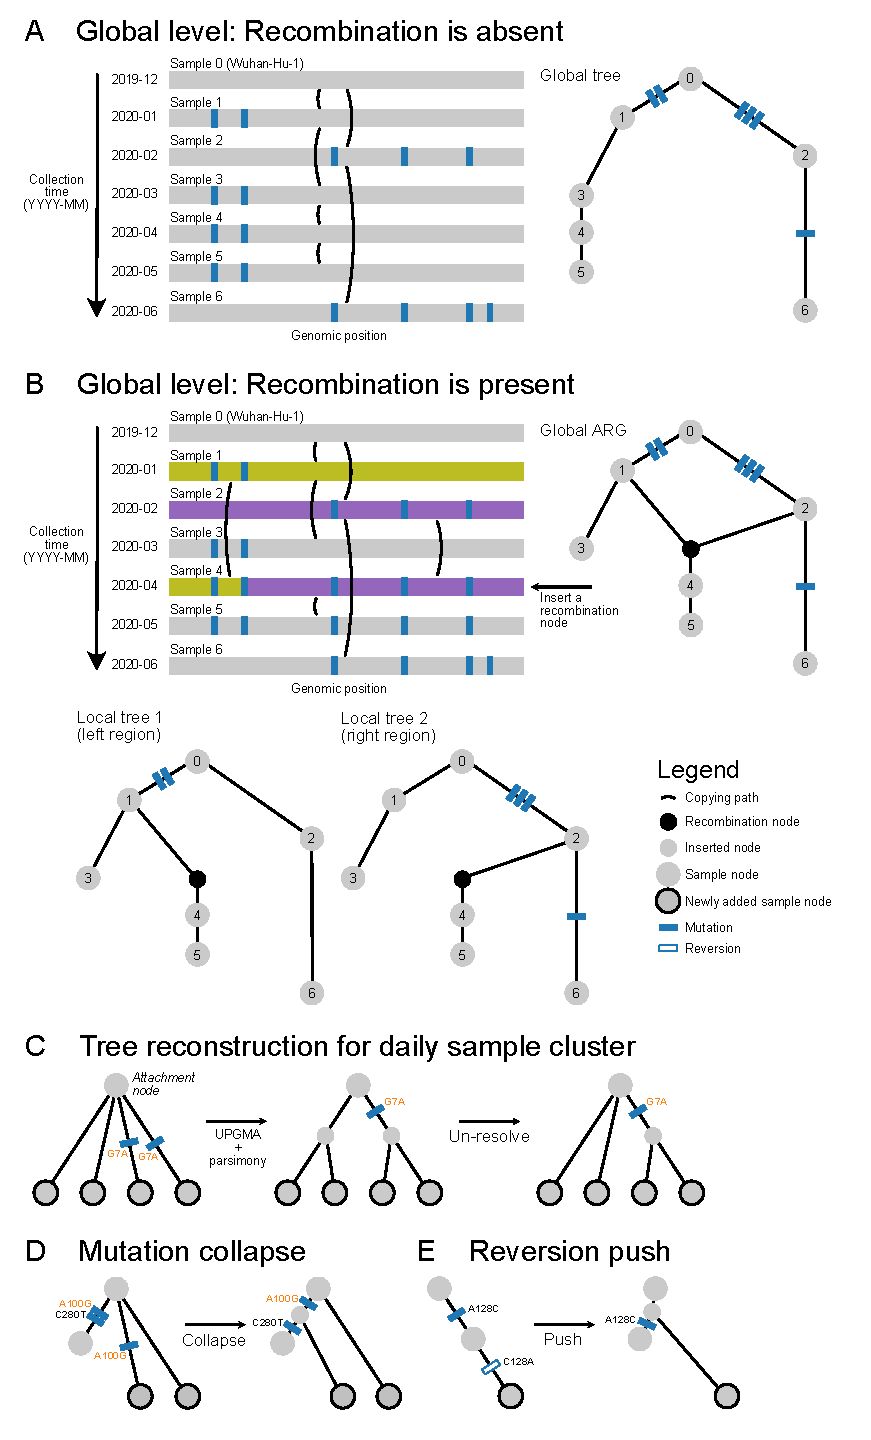
\includegraphics[width=0.7\textwidth]{figures/overview_sc2ts.pdf}
\caption{\label{fig:overview_sc2ts}
A schematic of the sc2ts method. Sc2ts reconstructs the genetic relationships
among SARS-CoV-2 genomes by copying samples to all possible ancestors collected
at earlier time points (curved arrows). An ARG is built by attaching new sample
genomes grouped by collection date to an existing ARG rooted at the Wuhan-Hu-1
reference genome, day by day. Each iteration involves three stages: (1)
attachment of new samples to the growing ARG (A, B); (2) reconstruction of
trees relating the samples under each attachment node (C); and parsimony-based
tree topology adjustments (D, E). In the absence of  recombination, sc2ts
infers an ARG that is a single tree relating the samples (A). However, in the
presence of recombination, sc2ts infers an ARG that is encoded as a sequence of
local trees relating segments of the sample genomes (B), inserting a
recombination node to represent a putative recombination event. Additionally,
mutation-collapsing nodes (D) and pushed-reversion nodes (E) are inserted to
make more parsimonious placements of mutations that should be shared or should
not be immediately reverted, respectively.}
\end{figure}


% We introduce an ARG inference method, summarised in
% Figure~\ref{fig:overview_sc2ts}.
% % Note going to rewrite this anyway, so not trying to make it flow.
% It uses (1) an efficient HMM implementation of the Li and Stephens (LS) model
% \citep{Li2003-ib} to copy SARS-CoV-2 genomes (see Sections 2.2 and 2.3); (2)
% the reported collection dates of the SARS-CoV-2 samples to determine the order
% of genome copying; and (3) several parsimony-based heuristics to locally refine
% the topology. In brief, this combined approach uses the likelihood model of LS
% to attach sample genomes to existing nodes and to detect recombinants, but
% because many of the daily tip samples harbour few, if any, mutational changes,
% we use parsimony to resolve their close relationships.

% Our HMM implementation, sc2ts, builds a reticulated graph for SARS-CoV-2 by
% taking advantage of the reported collection dates to incrementally grow the
% ARG. The inference process occurs forward in time, attaching new genomes
% aggregated by their collection date (daily batches), from the earliest to the
% last collection date. Prior to attaching sample genomes, the ARG is initialised
% such that the Wuhan-Hu-1/2019 reference genome is the root node. In the absence
% of recombination, the ARG is a single tree with no reticulation (Figure 1A);
% however, in the presence of recombination, a reticulate ARG is generated, with
% variation in tree topology across the genome (Figure 1B). Unlike standard
% phylogenetic trees in which internal nodes always represent inferred ancestors,
% internal nodes in the sc2ts ARGs represent sequences which can either be
% inferred ancestors or known samples.

% Each daily batch of genomes is first attached to the growing ARG without any
% phylogenetic resolution. In cases where the newly added sequence is inferred to
% be a recombinant, a recombination node is inserted; the ``date'' of this node
% is arbitrarily set to the average of the collection dates of the genome and the
% most recent of its parent nodes. Otherwise, the genomes are attached to the
% most closely related ancestral node (an attachment node). This creates
% polytomies that are then locally resolved among the descendants of each
% attachment node using the Unweighted Pair Group Method with Arithmetic Mean
% (UPGMA) algorithm \citep{Michener1957-tr}, with average linkage (Figure 1C).
% This hierarchical clustering algorithm produces a dendrogram relating a set of
% sequences, which is treated as an ultrametric binary tree here. Subsequently,
% mutations are placed onto the daily tree by maximum parsimony. An issue with
% the UPGMA algorithm is that it may create internal nodes supported by no
% informative site (i.e., having no mutation immediately ancestral to them). In
% an adjustment step, such unsupported internal nodes are removed to
% ``un-resolve'' the daily tree; the remaining internal nodes, which are
% supported by at least one shared mutation, are retained. The ``dates'' of the
% non-sample internal nodes are set to the same date as the samples in the daily
% batch. The resulting daily tree is grafted onto the attachment node in the
% global ARG.

% During ARG inference, two types of non-sample nodes are inserted to improve
% parsimonious placement of mutations: mutation-coalescing nodes and
% pushed-reversion nodes. We call these operations tree adjustments. A
% mutation-collapsing node is inserted when a shared mutation between sibling
% nodes is found (Figure 1D). An attempt to create mutation-collapsing nodes is
% made after grafting a new daily tree onto the global ARG. If shared mutations
% exist between two or more sibling nodes, then a parsimonious explanation is to
% create a new node that is the parent of those siblings, on which these
% mutations occurred. A pushed-reversion node is inserted when an immediate
% reversion occurs (Figure 1E), i.e. a mutation that reverts another mutation on
% its parent node. Instead of retaining both the mutation and immediate
% reversion, only the mutation is kept after a pushed-reversion node is inserted,
% thereby reducing the number of mutations on the branches. Note that these
% non-sample nodes are used as reconstructed genomes during HMM copying.

% Furthermore, during inference, the ARG is automatically encoded, stored, and
% updated as a tree sequence using tskit \citep{Kelleher2018-xc}.

\subsection{Ancestral Recombination Graphs}
The term ``Ancestral Recombination Graph'' was introduced by
Griffiths and colleagues~\citep{Griffiths1991-two,Griffiths1998-ancestral}
and originally defined an alternative formulation of the coalescent
with recombination stochastic process~\citep{Hudson1983-properties}.
Subsequently, the term ARG came to be used in a more general way to
describe not just realisations of this model, but to any
recombinant genetic ancestry~\citep{Minichiello2006-mapping}.
While there is some subtlety in the details~\citep{Wong2023-efficient},
we can think of an ARG as being any graph that encodes the
reticulate genetic ancestry of a sample of sequences under
the influence of recombination.

The ``succinct tree sequence'' is an ARG data structure
that is both general (in terms of the types of ancestry that can
be described) and computationally efficient~\citep{Wong2023-efficient}.
Originally developed to facilitate large-scale coalescent
simulations~\citep{Kelleher2016-wk}, the methods have been
extended and applied to forwards-time
simulations~\citep{Kelleher2018-xc,Haller2018-tree},
calculation of population genetics statistics~\citep{Ralph2020-efficiently}
and ARG inference~\citep{Kelleher2019-ba,Wohns2022-th}.
The succinct tree sequence is based on a simple tabular representation,
which defines a set of nodes, edges, sites and mutations. A \emph{node}
represents a particular genome, which may be an observed sample
or an inferred genetic ancestor. The genetic inheritance between
a pair of nodes along a segment of genome is defined by
the \emph{edge} $(\ell, r, p, c)$, which states that
child node $c$ inherited its genome from parent node $p$
from left coordinate $\ell$ to right coordinate $r$. A \emph{site}
defines the genomic position at which some variation occurs,
and a \emph{mutation} defines the site, node and derived state
that generates variation.
Given these tables, we can then efficiently construct the local
genealogical trees along the genome (arising from recombination),
and also perform a range of calculations efficiently by
reasoning about the differences between these local
trees~\citep{Kelleher2016-wk,Ralph2020-efficiently}. These
algorithms have led to peformance increases of several orders
of magnitude over the state-of-the-art in a range of
applications~\citep{Kelleher2016-wk,Kelleher2018-xc,Kelleher2019-ba,
Ralph2020-efficiently,Baumdicker2022-ep}.
The succinct tree sequence encoding
is also very concise, allowing, for example, for millions of
complete human genomes to potentially be stored in a few gigabytes of
space~\citep{Kelleher2019-ba}.

The \texttt{tskit} library~\citep{Tskit2023-tskit} is a liberally
licensed open source toolkit that provides a comprehensive suite
of tools for working with ARGs. Based on core functionality written
in C, it provides interfaces in C, Python and Rust. The Python interface
is based on NumPy~\citep{Harris2020-array}, and provides a convenient
platform for interactive analysis of large-scale data using, for
example, Jupyter notebooks~\citep{Kluyver2016-jupyter} and taking
advantage of the analysis tools in the burgeoning PyData ecosystem.
Tskit is mature software, widely used in population genetics, and
has been incorporated into several downstream
applications~\citep[e.g.][]{Haller2019-slim,Speidel2019-yh,
Terasaki2021-geonomics,
Fan2022-genealogical,Korfmann2022-weak,
Mahmoudi2022-bayesian,Petr2022-slendr,Rasmussen2022-espalier}.

\subsection{The Li and Stephens model}
\label{sec:ls}
The Li and Stephens (LS) model\citep{Li2003-ib}  is an approximation of the
coalescent with recombination~\citep{Hudson1983-properties}, which captures
many of the important features of the joint processes of mutation and
recombination. It is a Hidden Markov Model (HMM) in which a focal genome is a
sequence of nucleotides that are probabilistically emitted as
an imperfect mosaic of a set of reference genomes
(Figure~\ref{fig:ls_diagram}).
The LS model is used in a wide variety
of applications in genomics, including modern approaches to
statistical genotype phasing and imputation
\citep{Delaneau2019-wl,Browning2021-cg,Browning2018-nk,Rubinacci2020-pa},
and estimation of parameters such as
recombination rates \citep[e.g.][]{Hinch2011-tz},
and selection within and across hosts in viral
sequence data \citep[e.g.][]{Palmer2019-wa}.
See~\cite{Mcvean2019-linkage} for further review and discussion
of the LS model.

\begin{figure} \centering
\includegraphics[width=0.5\textwidth]{figures/ls_diagram_covid.pdf}
% FIXME this caption is too long
\caption{\label{fig:ls_diagram} A schematic of the Li and Stephens (LS)
model, in which a query sequence (bottom) is described as an
imperfect mosaic of the sequences in a reference panel.
Black crosses along the focal sequence show genotyping
errors or mutations.
In the standard formulation, at site $\ell$, the recombination probability is $r_\ell$,
the mutation probability is $\mu_\ell$ and $n$
denotes the size of the reference panel.
The Viterbi algorithm can be used to find a
``copying path'' through the reference panel for a given query sequence that
maximises the likelihood under these parameters.
% The LS HMM is governed by the transition and
% emission matrices, $Q$ and $E$, respectively.
% Each may be a function of the
% reference panel members, but transitions are generally assumed to be
% independent of the hidden states themselves (shown in the pink panel). This
% dramatically increases performance as the state space drops to two states
% (i.e., switching or not switching).
% Emissions may also be a function of the nucleotide states, but in our
% case, we assume that all observed alleles (in both the reference panel and
% focal sequence, $a\ell$) at the site under consideration are equally likely and
% occur with mutation probability $\ell$ (shown in the blue panel).
% These two
% processes, transition and emission (which encode recombination and mutation,
% respectively), define the generative process of the HMM, by which an imperfect
% mosaic is emitted from a reference panel.
 % of samples and nodes from the ARG
% inserted at earlier collection dates (shown in the lower panel). Here, the
% unseen states in the reference panel are shown as coloured lines enclosed by
% the grey box, and the true path through the data which leads to the emitted
% focal sequence is displayed by the black arrow. Examples of transition and
% emission probabilities along this trajectory are shown by the red and blue
% arrows, respectively.
% Note that in practice, we do not know the pattern of
% colours along the focal sequence and must infer it using the Viterbi algorithm.
}
\end{figure}

The generative process of the LS model is summarised in
Figure~\ref{fig:ls_diagram}. Here, a transition matrix, $Q$, governs the
process of switching (recombining) between members of the reference panel (the
hidden states). An emission matrix, $E$, allows for differences between the
focal sequence and the hidden state from which it is copied (due to mutation as
well as genotyping or sequencing error). Then, we use the Viterbi algorithm
\citep{Viterbi1967-ol} to find the most likely copying path through the
sequences, given a set of reference sequences, $Q$, and $E$.
The relative rates of mutation and recombination are usually controlled by
the site-specific parameters $\mu_\ell$ and $r_\ell$, respectively.
For this work we used a simpler formulation, which uses a single parameter
(the mismatch ratio, MMR) to control the relative importance of mutation
and recombination in the HMM. Specifically, an MMR value of $k$ will
prefer $k$ mismatches (mutations) to a recombination.[DUNCAN MORE DETAILS
HERE PLEASE]

[ALSO MENTION MISSING DATA, where we deal with Ns in the alignment]

% OLD text, ready to be adapted (and deleted once done)
% For this
% application, we have parameterised the HMM using a mismatch ratio (MMR), which
% tunes how strongly mutations (i.e., no switching of template sequences) are
% preferred over recombination (i.e., switching between sequences) during
% copying. Under a lower MMR value, the maximum-likelihood HMM copying path of a
% focal genome more likely spans at least two ancestral genomes (i.e,. the focal
% genome is a putative recombinant) than a single ancestral genome. Here, the MMR
% was set to three in all the HMM runs .

In \texttt{sc2ts} we use the efficient ARG-based implementation of the
LS Viterbi algorithm from \texttt{tsinfer}~\citep{Kelleher2019-ba} to find
the most likely copying path for each sample sequence
among all sequences (sampled and inferred) in the current ARG.
In the majority of cases, with non-recombinant sample sequences,
the most likely solution is to copy from one
of the nodes in the ARG that minimised the number of mutations required
on the query sequence. Importantly, because the reference panel here consists of
\emph{every} node in the ARG, we can match to both older sample
sequences or internal nodes representing an inferred ancestral sequence
(see subsequent subsections for details about how these are added).
Thus, when no recombination is present, the LS Viterbi algorithm is
implementing a version of parsimony, in which we are guaranteed to
find a sequence that minimises the number of additional mutations required
to incorporate a newly-added sample into the ARG.
Recombination is then inferred when the most likely solution to the LS
HMM is to copy from more than one ARG node along the genome, for a
given sample sequece. [TODO MORE]

We can solve this massive optimisation problem exactly because the ARG-based
implementation of the LS HMM used in \texttt{tsinfer} scales approximately
logarithmically with reference panel size (as opposed to linearly,
for standard matrix-based approaches)~\citep{Kelleher2019-ba}.
This efficient HMM algorithm is the main reason for \texttt{tsinfer}'s
scalability, and here allows us to find closely matching
sequences and recombination paths among millions of SARS-CoV-2
genomes exactly under a well-defined statistical model.

It is important to note that the Viterbi algorithm only returns
\emph{one of} the copying paths that maximise the likelihood under
 the given mutation and recombination parameters. There may be many
such paths, from which we choose one arbitrarily. Also, the
present choice of using a single mismatch-ratio parameter to control
the likelihood of recombination vs mutation may lead to relatively
flat likelihood spaces where many different paths have equal likelihood.
There are many possibilities in using established HMM methodology
to reason about and explore the space of possible matches, which may
be a fruitful avenue for future work. See the Discussion for further
potential improvements that may be made to the HMM.

\subsection{Tree inference from HMM daily sample clusters}
\label{sec:sample-cluster-tree-inference}
For a given daily batch of sample sequences that are to be attached to the
ARG, the LS HMM provides the most likely copying path and required mutations
for each of those sequences. We could directly attach these samples to
the ARG according to the copying paths and sets of mutations, but
such an approach would be highly unparsimonious because there are
often many samples that share the same copying path, with
complex patterns of shared mutations among those clusters of samples.
In this section we discuss the strategy used to infer likely tree
topologies within these clusters of samples sharing the same copying path.
In the majority of cases the copying path will consist of a single
node (i.e., no recombination), and so for simplicity we will assume in the
following discussion that all of the samples in a HMM-defined cluster
attach to a single node. The special treatment afforded to
newly-detected putative recombinants are discussed below
in Section XXX.

With tens of thousands of samples being added to the ARG per day,
we can have clusters of hundreds of sequences attaching to the same node.
While some of these samples will require no extra mutations
(i.e, they are identical to the attachment node), in general there
will be complex patterns of shared mutations among the samples
reflecting their evolutionary relationships. A natural way to infer
these within-cluster evolutionary relationships is to use standard
tree-building algorithms.
We can infer a likely tree relating the
samples in a cluster independently of the other samples in a
daily batch, and then attach the tree (and mutations)
to the ARG at the node identified by the HMM.

We currently use the implementation of the UPGMA algorithm~\citep{Michener1957-tr}
from SciPy~\citep{Pauli2020-scipy} to build trees from sample
clusters, and map mutations back to this topology using maximum parsimony.
This approach was chosen mainly for simplicity and because of the
speed and reliability of the implementation.
An issue with the UPGMA algorithm is that it generates a strictly
binary tree, creating internal nodes
supported by no informative site (i.e., having no mutation immediately
ancestral to them). To avoid such false precision we post-process
to remove unsupported internal nodes, representing the relationship
between $k$ identical descendants of the node as a polytomy of size $k$.

There are well-known issues with using such a simple algorithm for inferring
evolutionary relationships~\citep{Felsenstein2004-inferring}.
Since this within-cluster tree building has a significant influence on the
overall ARG topology (see Results), implementing more sophisticated
tree building methods which keep track of the location of the required mutations
(rather then inferring post-hoc by parsimony), is a likely avenue
for improvements in overall inference quality.

\subsection{Parsimony increasing heuristics}
\label{sec:parsimony-heuristics}
Attaching trees built from the clusters of samples that copy from
a particular node (or path of nodes for recombinants, see the
next section) under the HMM is an inherently greedy strategy,
and can produce inferences that are clearly unparsimonious.
The final step in adding a daily batch of samples to the ARG
is then to perform some local updates that target specific
types of parsimony violation in the just-updated regions of the
ARG. There are currently two parsimony-increasing operations
applied, which we refer to as ``mutation collapsing'' and ``reversion
pushing''.

Mutation collapsing inspects the siblings of a newly attached node
to check if any of them share (a subset) of the mutations that
it carries. If so, we increase the overall parsimony of the inference
by creating a new node representing the ancestor that carried
those shared mutations, and make that new node the parent of the
siblings carrying those shared mutations. The patterns of
shared mutations between siblings can be complex, and the current
implementation uses a simple greedy strategy for choosing
the particular mutations to collapse. [TODO back ref to the
Results section to discuss how important these nodes are]

The reversion push operation inspects newly added nodes to see
if any of its mutations are ``immediate reversions''; that is,
are reversions of a mutation that occured on the new node's
immediate parent. We increase the overall parsimony of the
inference by ``pushing in'' a new node in which descends from the
original parent which carries all its mutations except those
causing the reversions on the newly added node.
[TODO back ref to the
Results section to discuss how important these nodes are]

Together these operations substantially increase the overall parsimony
of the inferred ARGs, most noticably in terms of the number of
reversion mutations inferred. However, they are both simple
greedy operations, just examining the local parts of the
ARG topology affected by newly added samples. Since the inferred
ARGs still contain a large number of reversion mutations which
are likely to be mostly artefactual, it is clear that there
is room for improvement, and that further parsimony increasing
heuristics would likely be of benefit.

\subsection{Treatment of recombinants}
A sample sequence is designated as a recombinant if the most likely
path inferred by the LS HMM for that sample contains at least
one switch between parents. Recombinant sequences are mostly treated
identically to non-recombinants, as we simply need to reason about
a path of parent nodes along genome intervals rather than a
single parent over the whole genome, which is naturally handled by
the succinct tree sequence data structure and \texttt{tskit} library
(see the Ancestral Recombination Graphs section above). To facilitate
analysis and to help understand the robustness of recombinants
we perform some additional steps in \texttt{sc3ts}.

The LS HMM may infer identical paths and patterns of mutations
for multiple samples in a daily batch, and so we
create a ``recombination`` node (marked with a specific ``flags'' value)
for each distinct recombinant. (This node is not strictly necessary
but makes it convenient to find recombinants for subsequent analysis.)
Variation within a cluster
of recombinant sequences is handled in the same way as non-recombinants
(see Section~\ref{sec:sample-cluster-tree-inference} above for details).

When the Viterbi algorithm implementation used by the LS HMM infers
recombinant ancestry for a given genome, the point at which inheritance
switches from one parent node to another is the last possible
position.
Thus, the breakpoints used in the ARG represent the rightmost end of the
interval, within which the recombination event could have occurred. To obtain
the leftmost end of this interval, we rerun the HMM using mirrored coordinates
(i.e., from the 3’ end to the 5’ end) and store the information as
metadata on the recombination node.
These left- and rightmost positions
are the recombination intervals reported throughout.
Ultimately all the recombination intervals mean is that the parent sequences
are identical within that interval, and there is therefore no information
about where the recombination occured. There are many different processes
that can contribute to the size of these intervals, and therefore
understanding how these processes interact to produce wider or narrower
intervals is an important avenue for future work.

The LS HMM machinery, and the interpretation of inferred recombinant paths and
breakpoint intervals is a central part of \texttt{sc2ts}, and there are many
ways to extend and improve. For example, the current parameterisation of using
a single ``mismatch ratio'' is very simplistic (see section XXX), and likely
results in a very flat likelihood space where many sequences have equal
likelihood of being chosen. More sophisticated parameterisations where we
condition on known per-site mutation rates (and perhaps per-base subsitution
rates) may lead to better results, although perhaps at the cost of some
reduction in interpretability. Post-processing the match results to produce
more parsimonious breakpoints may also be a worthwhile avenue for development.
In particular, we may choose to insert breakpoints for the ARG that are choosed
from within the possible interval, rather than the current approach of taking
the right-most value. Cases where we have more than two parents may either be
the ``stacking'' of multiple recombination events, or instances where
the HMM has chosen to switch to a third sequence rather than back to
the original parent (where this is equally parsimonious). Many putative
recombination events, however, will represent poor quality data, where
a recombinant copying path happens to be a more likely explanation
of a highly divergent sequence.
A thorough analysis of the behaviour of the LS model in the context
of a pandemic-scale ARG may lead to significant improvements in our
ability identify recombinants and to filter poor quality data.

\subsection{Node dating}
The approaches to assigning a date to nodes in \texttt{sc2ts} is currently
ad-hoc, and the inferred timing of events from the ARGs reported
here should be treated with caution (e.g., Figure~\ref{fig:recomb_mrcas}).
Sample nodes (those corresponding to observed sample sequences) are the
most accurately dated, as we use the reported collection date for
these nodes. These are not entirely accurate, but our data filtering
criteria should remove the most egregious errors (see
Section~\ref{sec:filtering_time_travellers}). Other nodes in the ARG
are dated by splitting the time between the attached samples
and the chosen parent nodes equally (in the case of
trees inferred from daily sample clusters,
Section~\ref{sec:sample-cluster-tree-inference}) or by adding arbitrary
small values when creating new nodes using parsimony rules
(Section~\ref{sec:parsimony-heuristics}). Substantial improvements could
likely be made using simple node dating methods.

\subsection{Data preprocessing}
The findings of this study are
based on sequences and metadata available on GISAID (\url{https://gisaid.org/})
up to Aug 22, 2022 and accessible at
\url{https://doi.org/10.55876/gis8.230329cd} (Supplementary Table 1).
We removed sequences
if they (1) had ambiguous collection dates;
(2) were collected before January 01, 2020 or after June 30, 2022; or
(3) were isolated from a non-human host.
We aligned sequences to the Wuhan-Hu-1/2019 reference sequence
(GenBank: MN908947.3) using Nextclade v2.3.0~\citep{Aksamentov2021-hj} (dataset tag
2022-07-26T12:00:00Z). We also excluded sequences if they had a
``bad'' quality control status
in any of the four Nextclade columns (``qc.missingData.status'',
``qc.mixedSites.status'', ``qc.frameShifts.status'' and `qc.stopCodons.status'').

We encode ambiguous nucleotide letters (i.e.,
not A, C, G, T, or a gap) in the pairwise genome alignments as missing data
(N). Problematic bases in the alignments, which had two or more Ns or
gaps within a distance of seven bases, are masked as missing data following
the approach used in the ``faToVCF`` tool used by
UShER~\citep{Turakhia2022-it}.
Sites that are masked by this process are
treated as missing data by the LS HMM (Section~\ref{sec:ls}).
In addition, we exclude 481 problematic sites flagged as prone to
sequencing errors or as highly homoplasic
(\url{https://github.com/W-L/ProblematicSites_SARS-CoV2/},
accessed 2022-09-22) entirely.

Although the masking strategy used currently is simple and robust,
there are significant disadvantages, excluding, for example, any
deletions of length greater than one base. Exploring more sophisticated
masking strategies is an important route for future improvements.

\subsection{Filtering ``time travellers''}
\label{sec:filtering_time_travellers}
A major source of error in early versions of \texttt{sc2ts} was
the existance of ``time traveller'' sequences: those with erroneously
early collection dates.
For example, an Alpha sample purportedly collected in 2020 from the United States,
before Alpha appeared in the United Kingdom (USA/MN-Mayo-1563/2020)
produced significant topological distortions in
ARGs inferred early on in the study.
Hence, to exclude such potential ``time travellers'' we employ two filters.
The first is to remove any sequence with a collection date that pre-dates the
time to the most recent common ancestor (tMRCA) of its corresponding clade.
We obtained the tMRCA for each clade from a Nextstrain GISAID reference tree
(downloaded on August 22, 2022), and we used the lower bound of the 95\%
confidence interval of each clade as the minimum date cut-off.
This removed NN [Katherine can you fill in please?] sequences.

This filter removes the most egregious time travellers, but many still
remain. We thus employed a second filter which is a simple threshold on
the time delay between the collection date and submission date.
After some preliminary analysis we settled on a maximum submission delay
of 30 days when building the ARGs described here as a reasonable compromise.

As the results of \texttt{sc2ts} are sensitive to the existance of
time-travellers, an imporant aspect of future work is to find better ways
to identify them. One possibility is to use the LS HMM itself to flag
overly divergent sequences, and to exclude them from attachment to the ARG.
We might also estimate collection dates by adding these potential time travellers
back to the ARG, allowing an automated assessment of collection date discrepancies.

\subsection{Imputation of Pango lineage for non-sample nodes}
% FIXME the caption and the text are basically saying the same thing here. Can
% we streamline, and maybe give a bit more detail in the text about iteration,
% and the concrete implementation?
\begin{figure} \centering
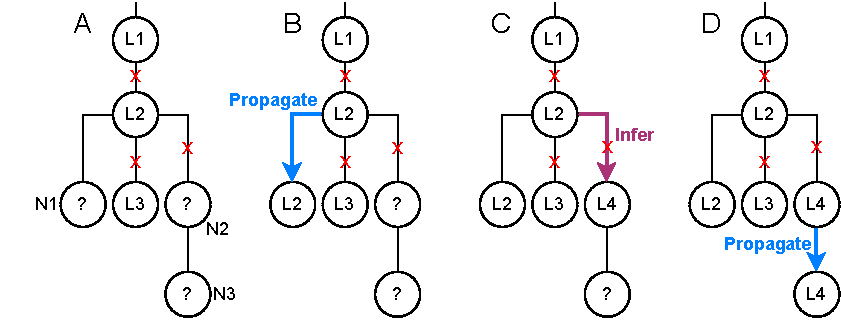
\includegraphics[width=.7\textwidth]{figures/imputation.pdf}
\caption{\label{fig:imputation}A schematic of the two-step procedure to impute
Pango lineage for inserted, non-sample nodes. Here, three nodes (question
marks) have unknown Pango lineage (A). Because the parent of node 1 is
available (i.e., L2) and there is no mutation occurring on the edge connecting
the two nodes, the Pango lineage of the parent is directly propagated to node 1
(B). However, if there is a mutation (red X’s), then the Pango lineage is
inferred by comparison to the set of lineage-defining mutations from
COVID-CG\citep{Chen2021-zc}, as in case (C). Finally, the inferred status is
propagated to any non-mutant child nodes, as in case (D).
}
\end{figure}
For many applications it is helpful to infer the Pango lineage status
of the internal ARG nodes estimated by \texttt{sc2ts}.
% Initially, only sample nodes have Pango lineage assignments.
% For analysis of recombinant parents, it is also helpful to assign
% Pango lineages to non-sample nodes.
We do this using a two-step procedure (Figure~\ref{fig:imputation}).
Initially, only sample nodes have Pango lineage assignments.
For a given non-sample node $u$, if the Pango lineage of its parent is
available and there are no intervening mutations,
then we impute that $u$'s Pango lineage is the same as its parent.
Otherwise, the Pango lineage of the
non-sample node is inferred by matching its full set of mutations against the
Pango lineage-defining mutations (based on 90\% consensus of the sequences
analysed) from the COVID-CG website \citep{Chen2021-zc};
\url{https://covidcg.org/}; accessed on November 04, 2022).

[TODO how accurate is this approach? We should probably discuss it somewhere
in the Results, and refer back from here? ]

\section{Acknowledgements}
We gratefully acknowledge all data contributors, i.e., the Authors and their
Originating laboratories responsible for obtaining the specimens, and their
Submitting laboratories for generating the genetic sequence and metadata and
sharing via the GISAID Initiative, on which this research is based. Also, we
thank Dr. Morag Graham (the National Microbiology Laboratory, Winnipeg, Canada)
for kindly providing the genomic coordinates of the breakpoint sequence motifs.
SHZ is supported by the Janssen-Oxford Translational Genomics Fellowship. JK,
YW, and BJ are supported by the Robertson Foundation.

\section{Data Availability}
The source code for \texttt{sc2ts} is
is available on GitHub
\url{https://github.com/jeromekelleher/sc2ts/}.
The Jupyter notebooks and code used to produce the results described here are also
available on GitHub \url{https://github.com/jeromekelleher/sc2ts-paper/}.

% TODO what's the right way to say this?
The inferred ARGs described here are available on request to those with
the appropriate GISAID data access.

\bibliographystyle{plainnat}
\bibliography{paper}

\renewcommand\thefigure{S\arabic{figure}}
\setcounter{figure}{0}
\renewcommand\thetable{S\arabic{table}}
\setcounter{table}{0}
\section*{Supplementary}

\begin{figure} \centering
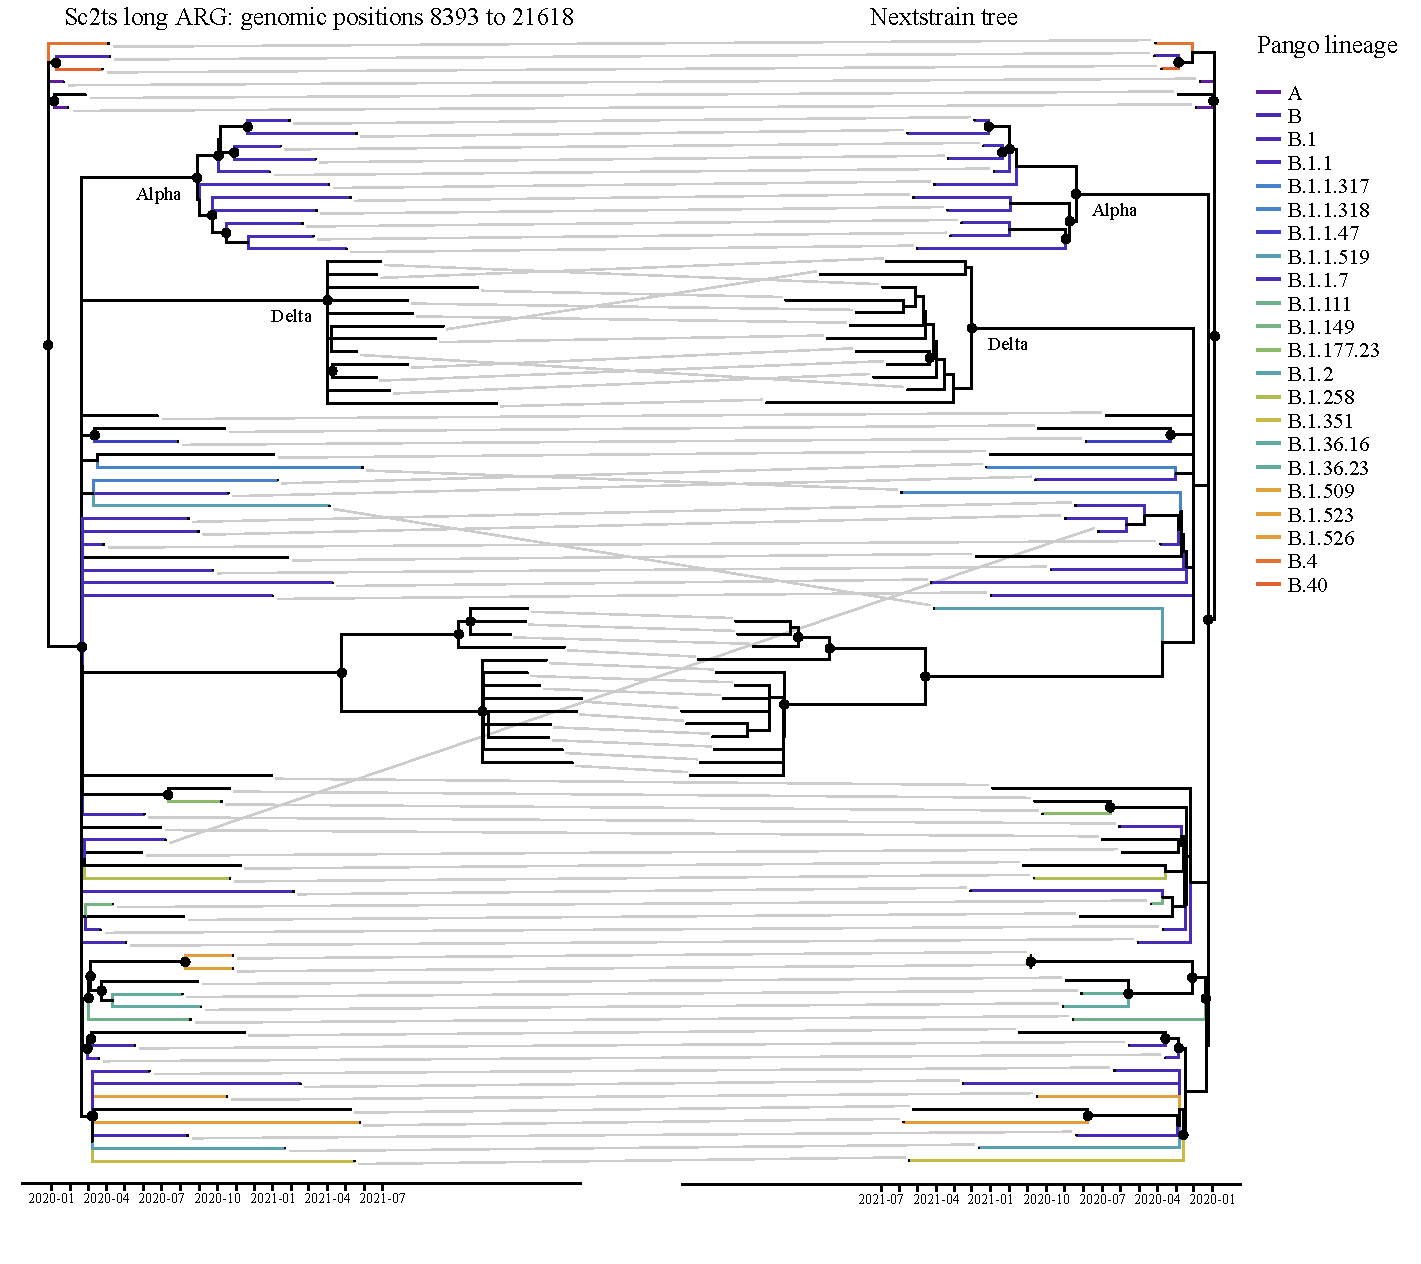
\includegraphics[width=\textwidth]{figures/supp_cophylogeny_long.pdf}
\caption{\label{fig:cophylogeny_long}Tanglegram equivalent to that in Figure~\ref{fig:cophylogeny}, but for the long ARG (i.e. subsampled to mid-2022). }
\end{figure}

% FIXME there's too much vspace between the rows here. Probably best to redo
% the formatting.
\begin{table} \centering
\begin{tabular}{l|c|c|c|c|c} \hline
\multicolumn{1}{c}{} & \multicolumn{3}{c}{\textbf{Jackson et al. (2021)}} &
\multicolumn{2}{c}{\textbf{sc2ts (wide ARG)}} \\ \hline
\textbf{Sample} &
\textbf{Group} & \textbf{Parents} & \thead{Breakpoint \\
interval(s)} &
\textbf{Parents} & \thead{Breakpoint \\ interval(s)} \\
\hline ALDP-11CF93B & A
    & \thead{B.1.177 \\ Alpha} & 21,255–21,613 & \thead{B.1.177.18 \\ Alpha} &
21,256–22,227 \\
    ALDP-125C4D7 & A & \thead{B.1.177 \\ Alpha} & 21,255–21,613 &
    \thead{B.1.177.18 \\ Alpha} & 21,256–22,227 \\
ALDP-130BB95 & A & \thead{B.1.177 \\ Alpha} & 21,255–21,613 &
    \thead{B.1.177.18 \\ Alpha} & 21,256–22,227 \\
LIVE-DFCFFE & A & \thead{B.1.177 \\ Alpha} & 18,998–20,294 &
    \thead{B.1.177.18 \\ Alpha} & 21,256–22,227 \\
QEUH-CCCB30 & B & \thead{B.1.36.28 \\ Alpha} & 6,528–6,953 &
    \thead{B.1.36 \\ Alpha} & 6,529–6,954 \\
QEUH-CD0F1F & B & \thead{B.1.36.28 \\ Alpha} & 6,528–6,953 &
    \thead{B.1.36 \\ Alpha} & 6,529–6,954 \\
MILK-1166F52 & C & \thead{Alpha \\ B.1.221.1} & 25,996–27,441 &
    \thead{Alpha \\ B.1.221} & 25,997–27,972 \\
MILK-11C95A6 & C & \thead{Alpha \\ B.1.221.1} & 25,996–27,441 &
    \thead{Alpha \\ B.1.221} & 25,997–27,972 \\
QEUH-109B25C & C & \thead{Alpha \\ B.1.221.1} & 25,996–27,441 &
    \thead{Alpha \\ B.1.221} & 25,997–27,972 \\
MILK-126FE1F & D & \thead{B.1.36.39 \\ Alpha} & 20,703–23,062 &
    \thead{B.1.36.39 \\ Alpha} & 22,445–23,063 \\
RAND-12671E1 & D & \thead{B.1.36.39 \\ Alpha} & 20,703–23,062 &
    \thead{B.1.36.39 \\ Alpha} & 22,445–23,063 \\
RAND-128FA33 & D & \thead{B.1.36.39 \\ Alpha} & 20,703–23,062 &
    \thead{B.1.36.39 \\ Alpha} & 22,445–23,063 \\
CAMC-CBA018 & n/a & \thead{B.1.177 \\ Alpha} & 20,389–21,254 &
    \thead{B.1.177 \\ Alpha} & 16,177–21,255 \\
CAMC-CB7AB3 & n/a & \thead{Alpha \\ B.1.177 \\ Alpha} & \thead{3,267–4,474 \\ 20,389–21,254} &
     \thead{Alpha \\ B.1.177 \\ Alpha} & \thead{3,268–5,388 \\ 16,177–21,255} \\
MILK-103C712 & n/a & \thead{B.1.177.17 \\ Alpha} & \thead{408–444 \\ 26,801–27,876} &
    n/a & n/a \\
QEUH-1067DEF & n/a & \thead{Alpha \\ B.1.177.9} & 10,523–10,869 &
    \thead{Alpha \\ B.1.177} & 7,729–10,870 \\ \hline
\end{tabular}
\caption{\label{tab:jackson_supplement}Recombinant sequences involving the Alpha (B.1.1.7) variant reported by \cite{Jackson2021-ik} have recombinant ancestry in the wide ARG. The breakpoint intervals and Pango lineage assignments of the parents were taken from Table 2 (3SEQ results) of Jackson et al., except the Pango lineage assignment of the parents of group B recombinants, which were taken from Table 1 (motif-based results).}
\end{table}

\begin{figure} \centering
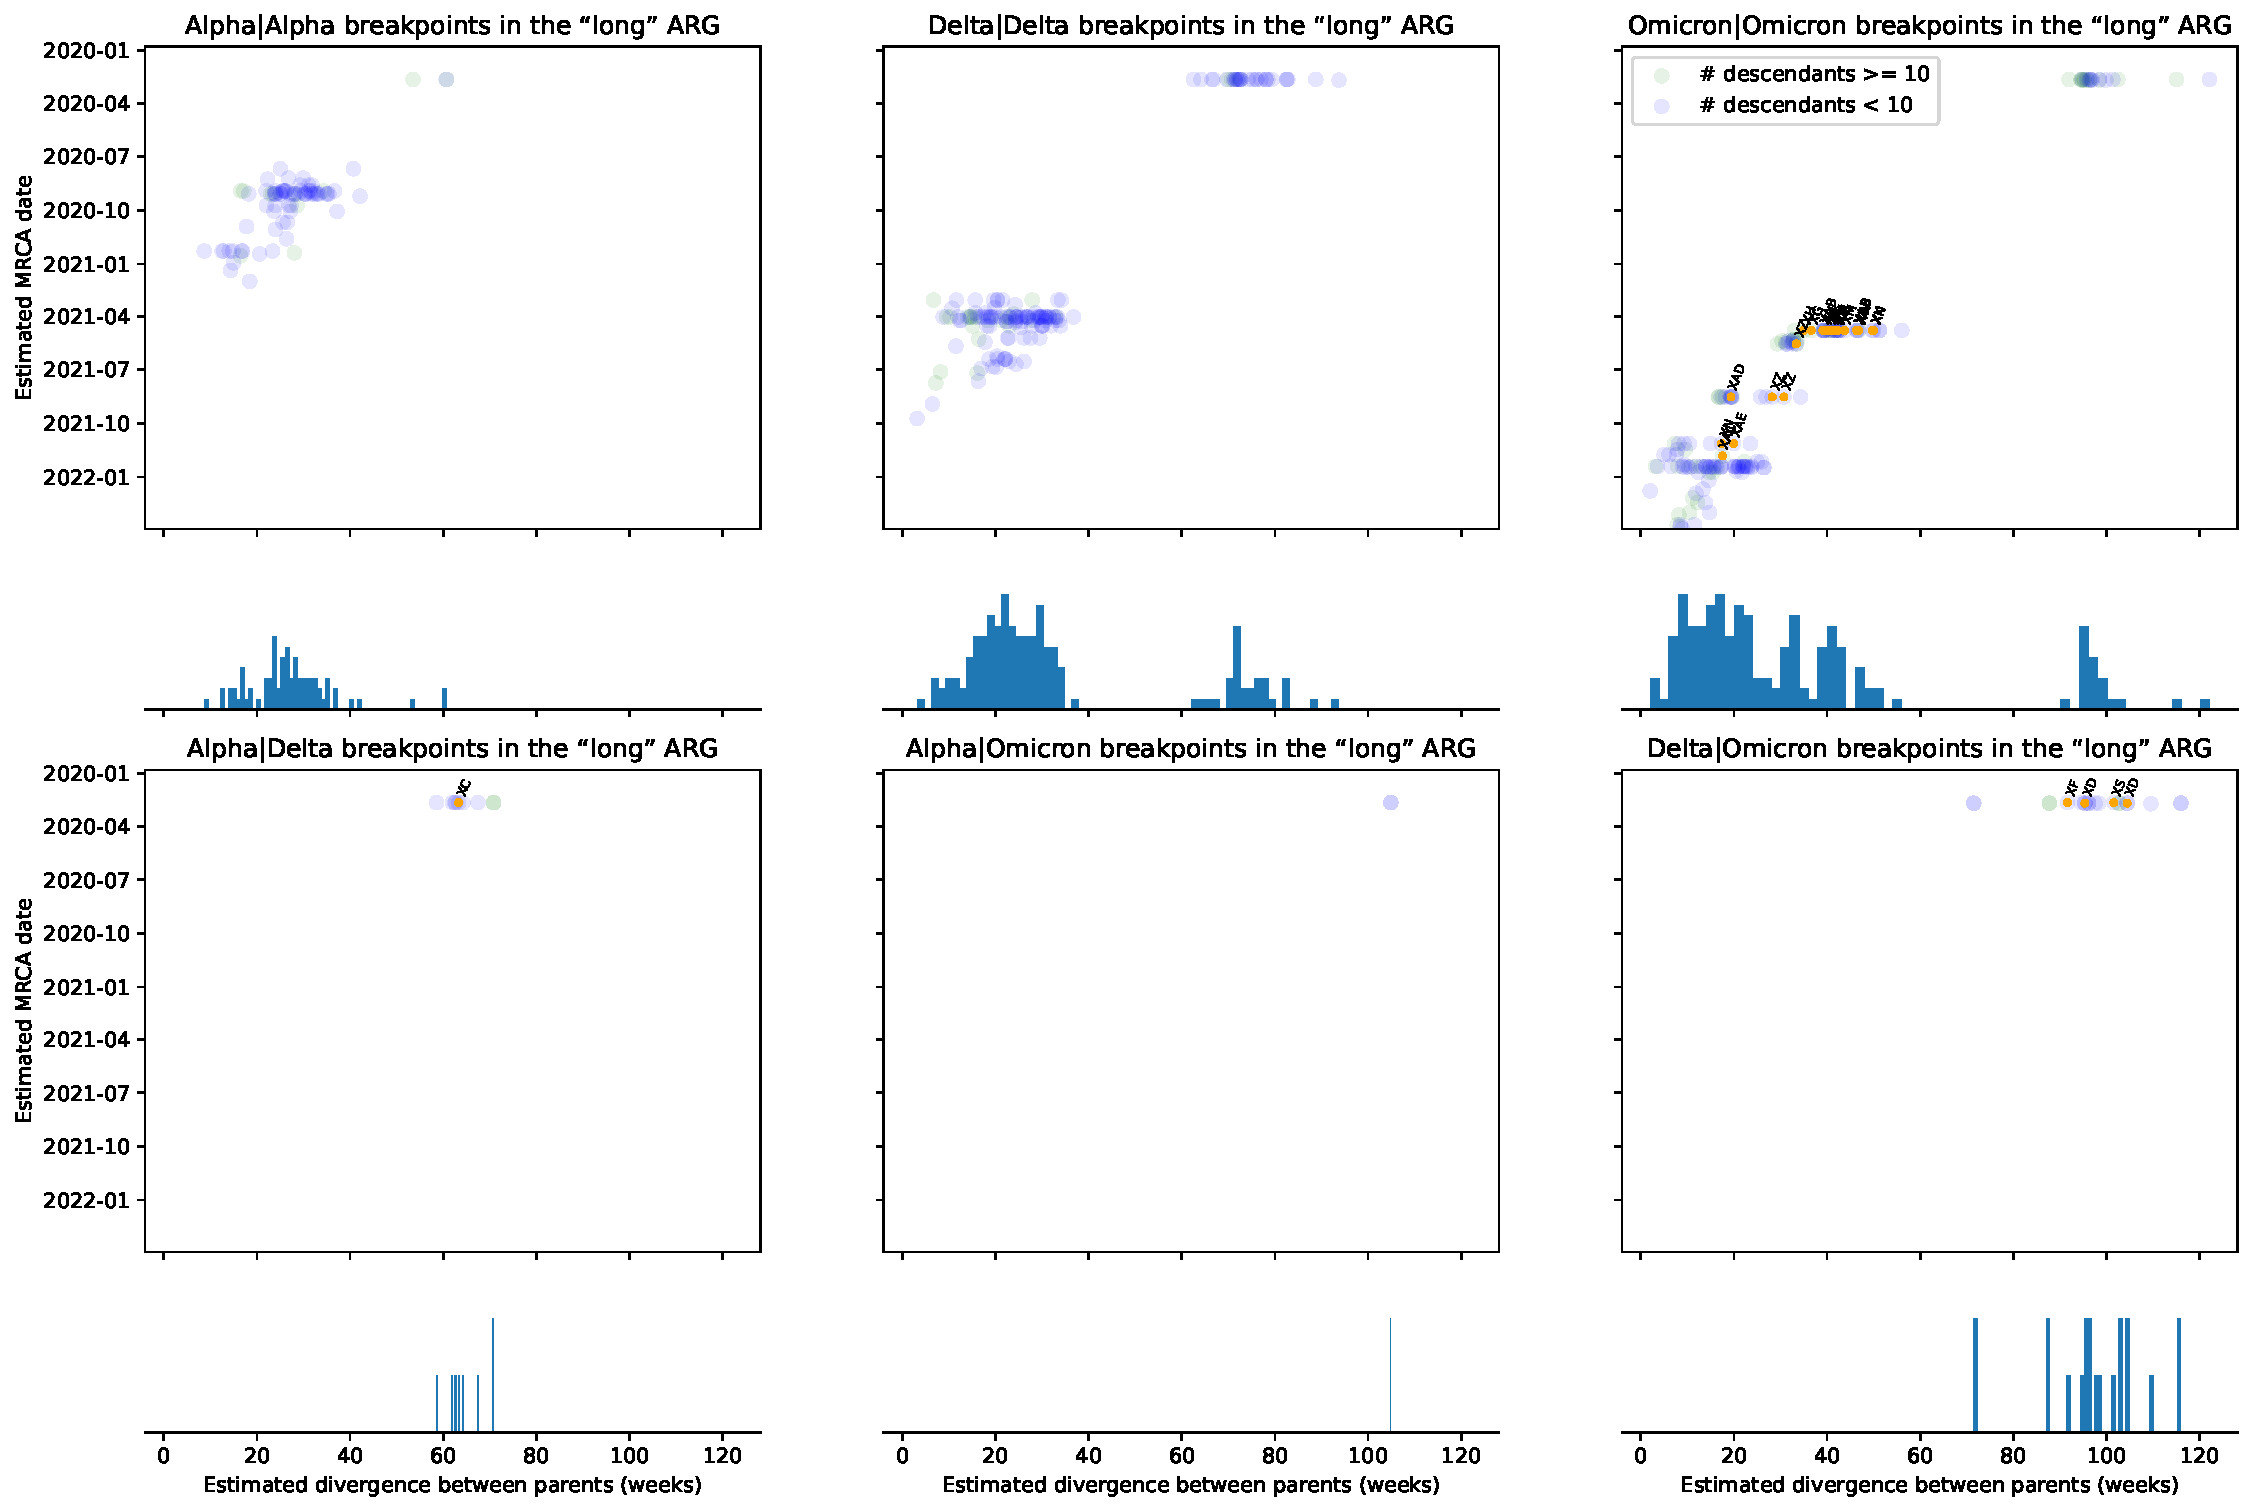
\includegraphics[width=\textwidth]{figures/supp_recombination_node_mrcas.pdf}
\caption{\label{fig:recomb_mrcas_voc_breakdown}  Divergence between parent lineages for recombination events within and among different VoC categories. HMM-consistent recombinants are shown in green, HMM-inconsistent in blue (including many of the named Delta-Omicron recombinants). We find 69 HMM consistent (77 inconsistent) Alpha-Alpha recombination breakpoints = 13\% (10\%) of the total; 84 HMM consistent (143 inconsistent) Delta-Delta recombination breakpoints = 18\% (18\%) of the total; 99 HMM consistent (155 inconsistent) Omicron-Omicron recombination breakpoints = 22\% (19\%) of the total; and 2 HMM consistent (20 inconsistent) Delta-Omicron recombination breakpoints = 2\% (< 1\%) of the total. These plots do not include recombination breakpoints involved lineages that were not classified into these VoC categories}
\end{figure}

\begin{figure} \centering
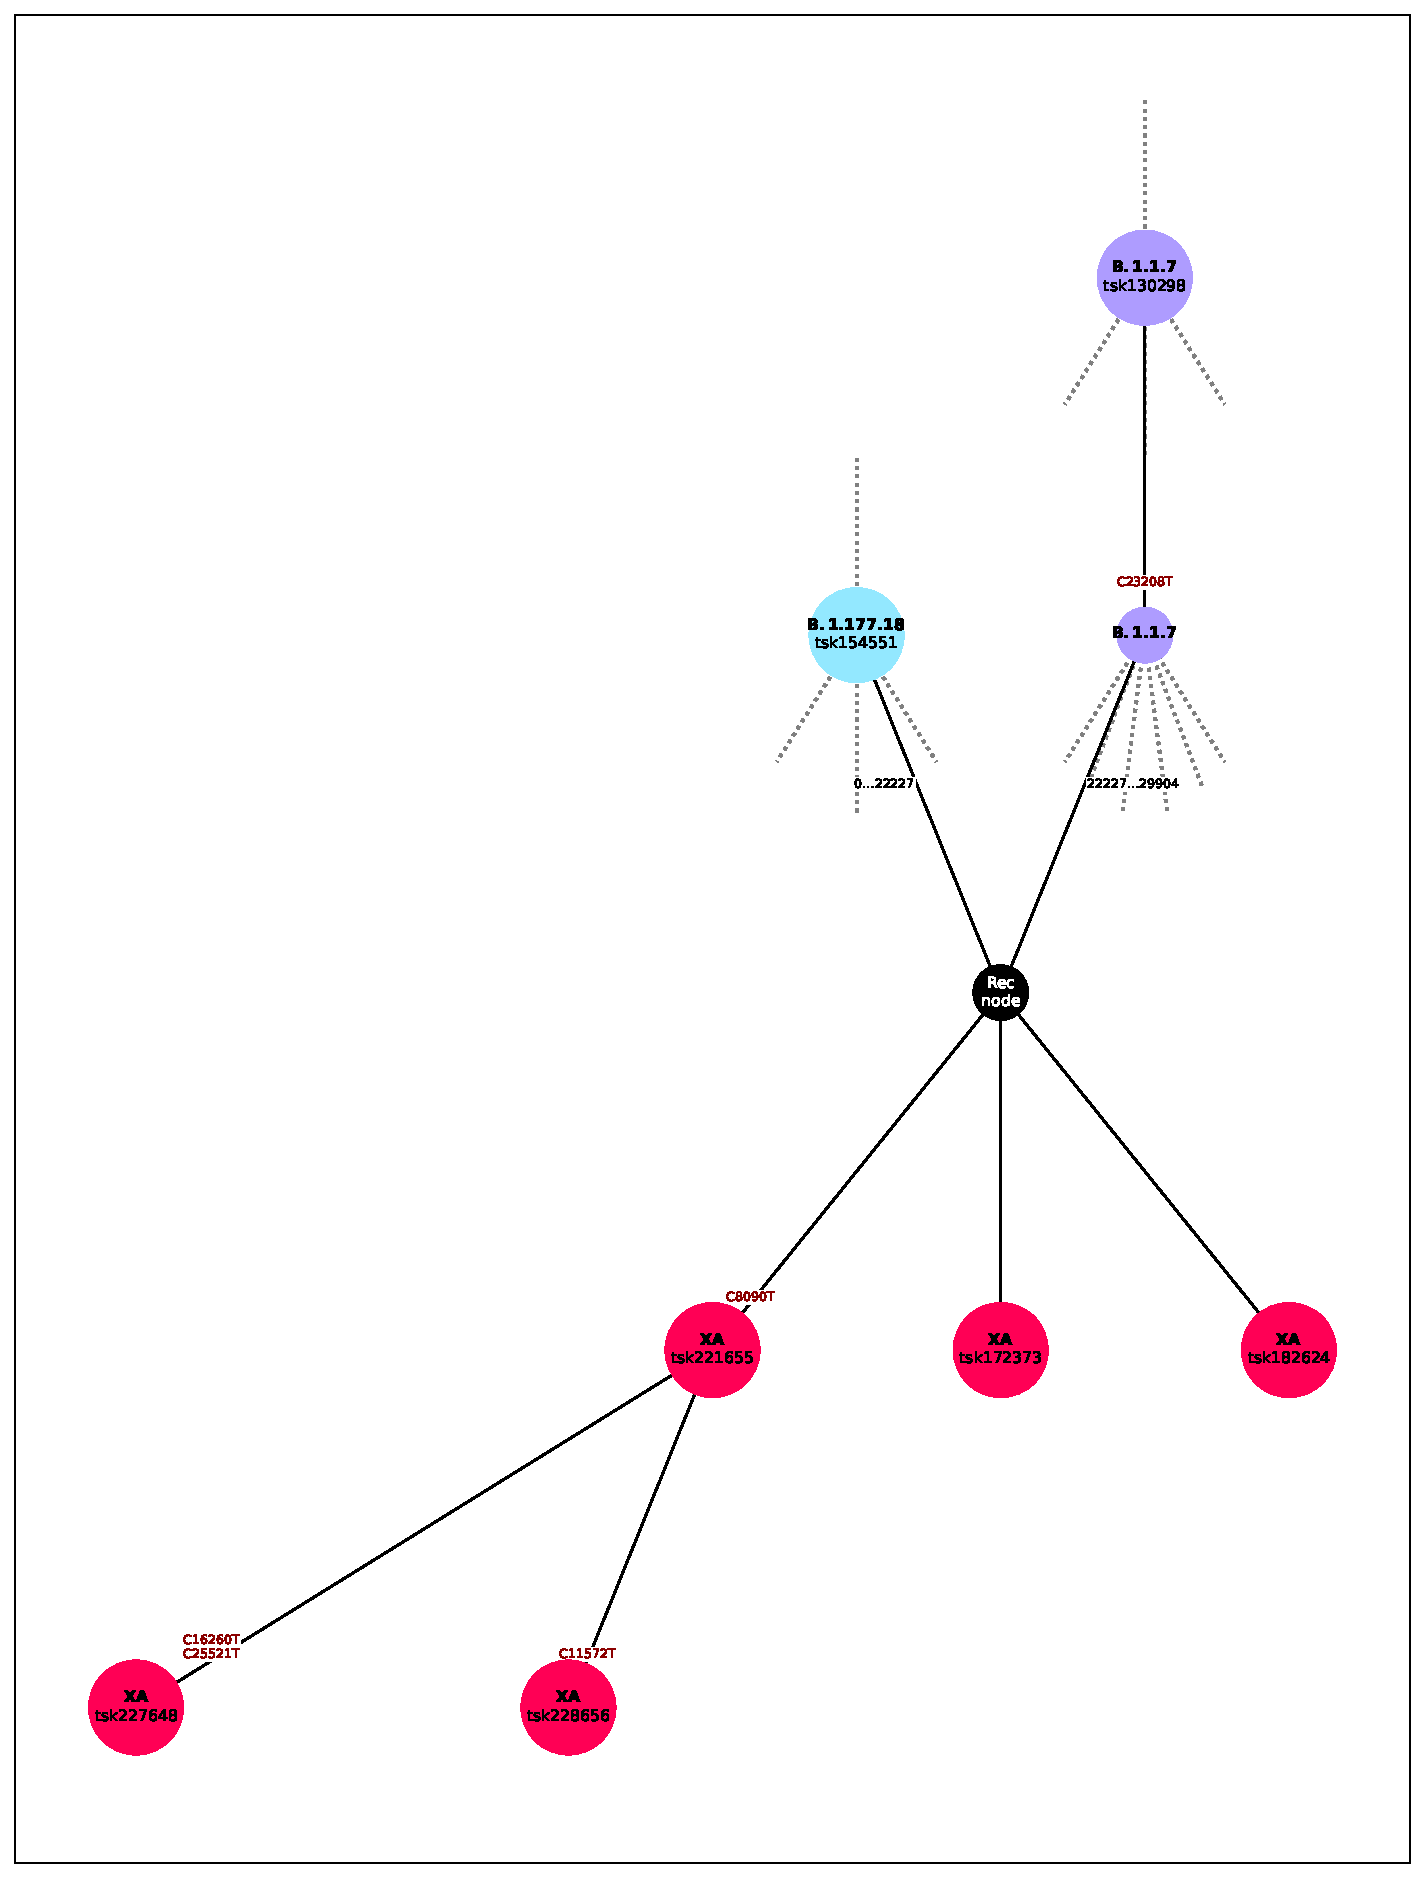
\includegraphics[width=\textwidth]{figures/Pango_XA_gisaid_large_graph.pdf}
\caption{\label{fig:pango_XA_gisaid_graph}  DESCRIBE ME}
\end{figure}

\begin{figure} \centering
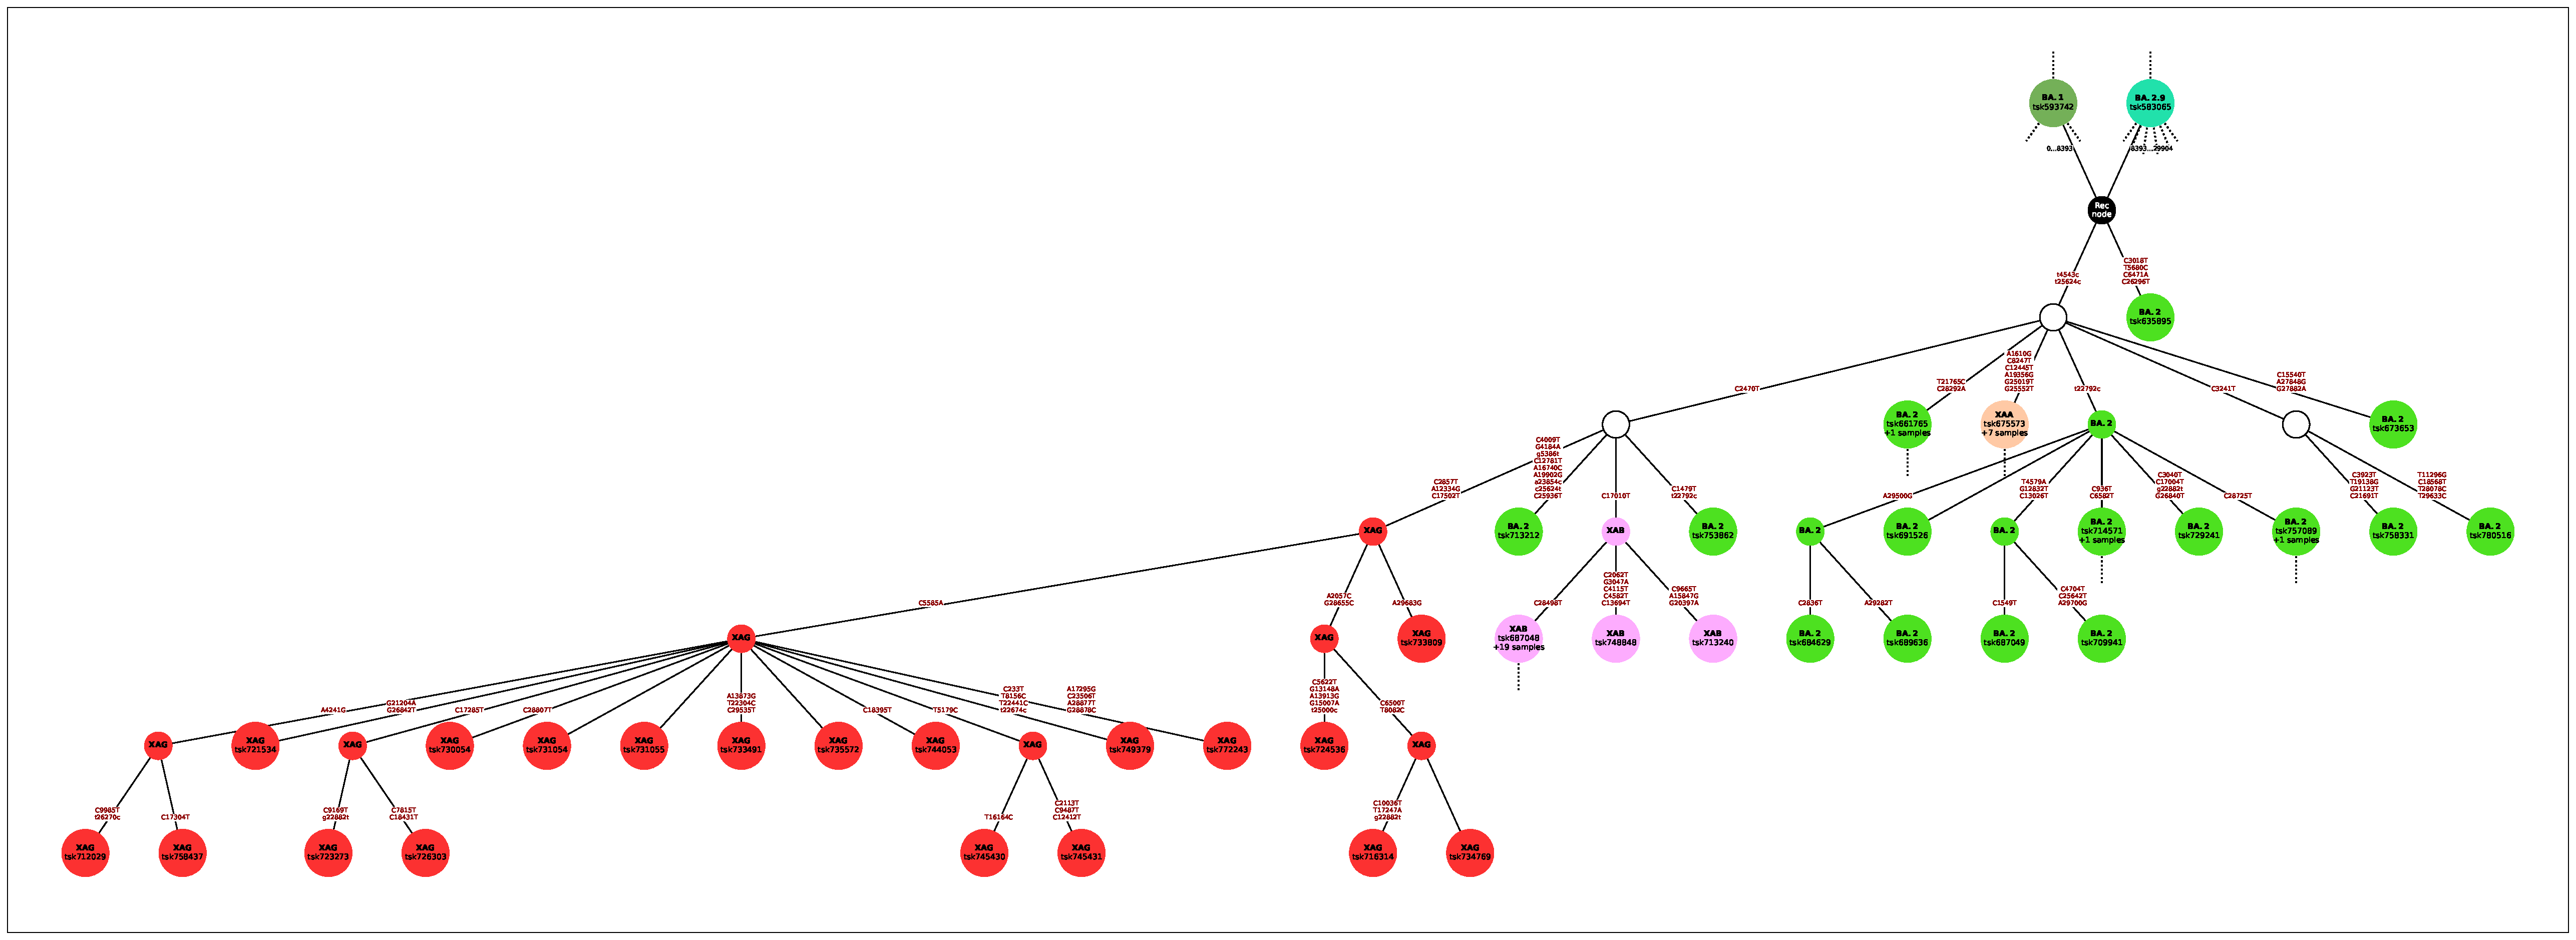
\includegraphics[width=\textwidth]{figures/Pango_XAG_gisaid_large_graph.pdf}
\caption{\label{fig:pango_XAG_gisaid_graph}  DESCRIBE ME}
\end{figure}

\begin{figure} \centering
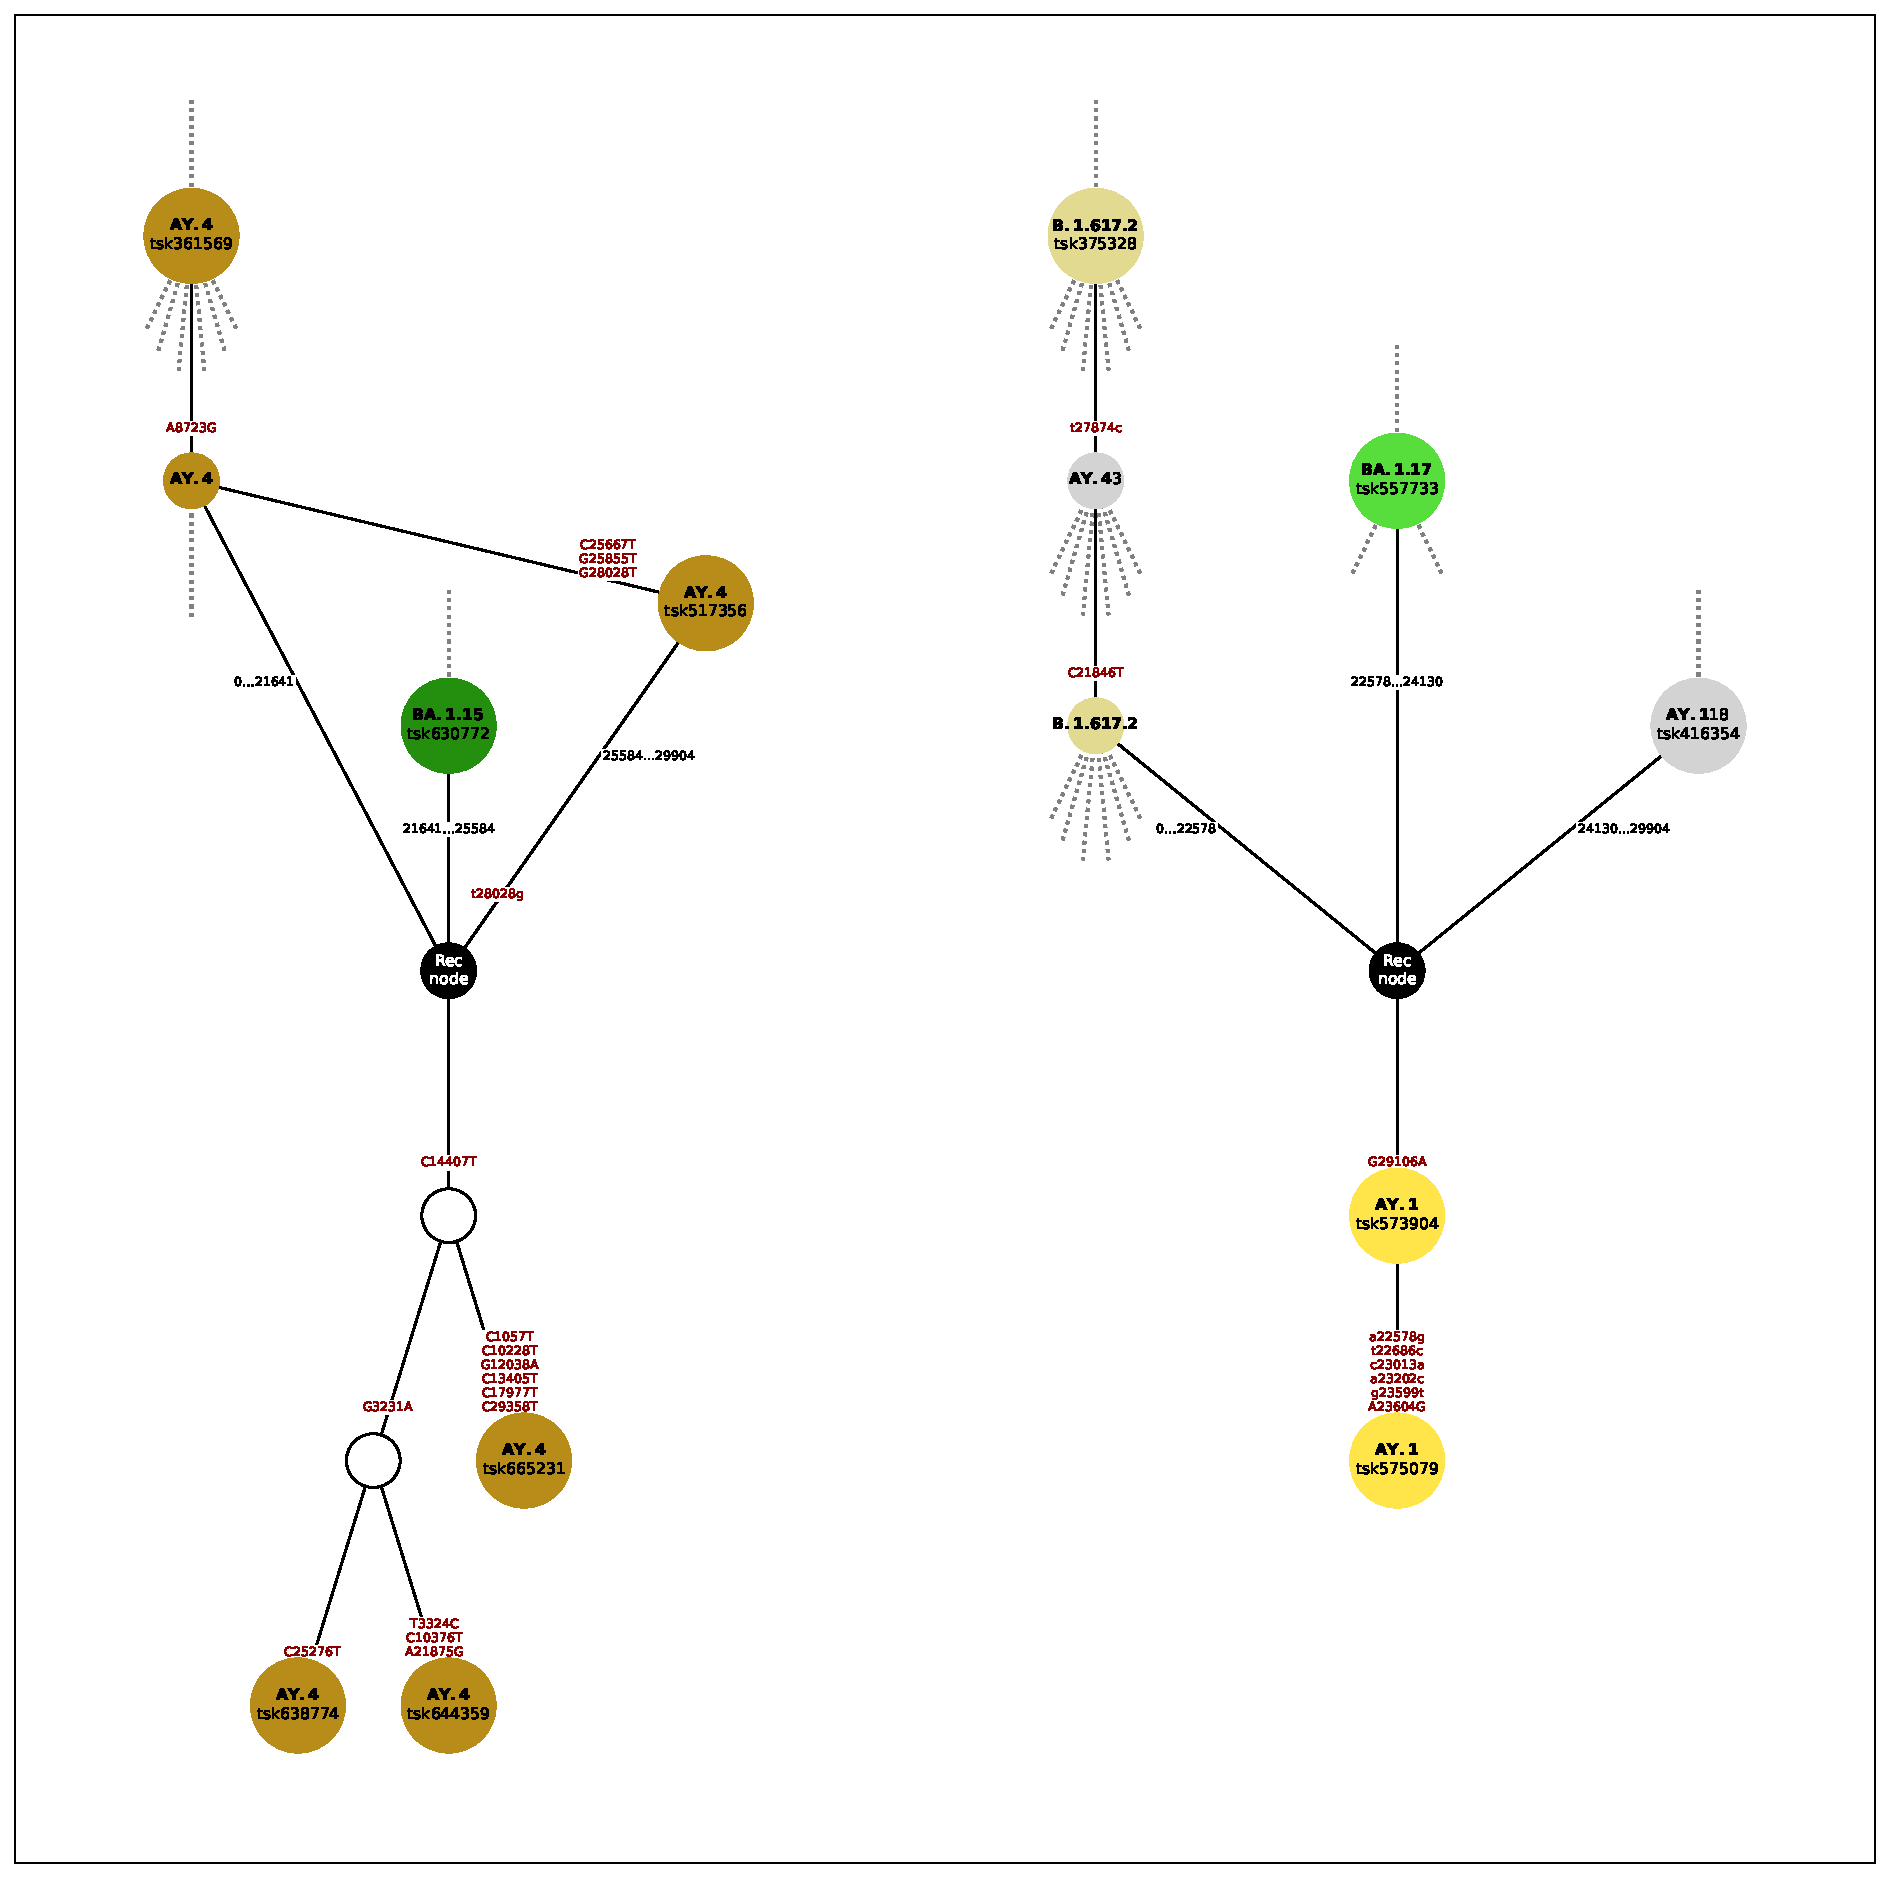
\includegraphics[width=\textwidth]{figures/Pango_XD_gisaid_large_graph.pdf}
\caption{\label{fig:pango_XD_gisaid_graph}  DESCRIBE ME}
\end{figure}

\begin{figure} \centering
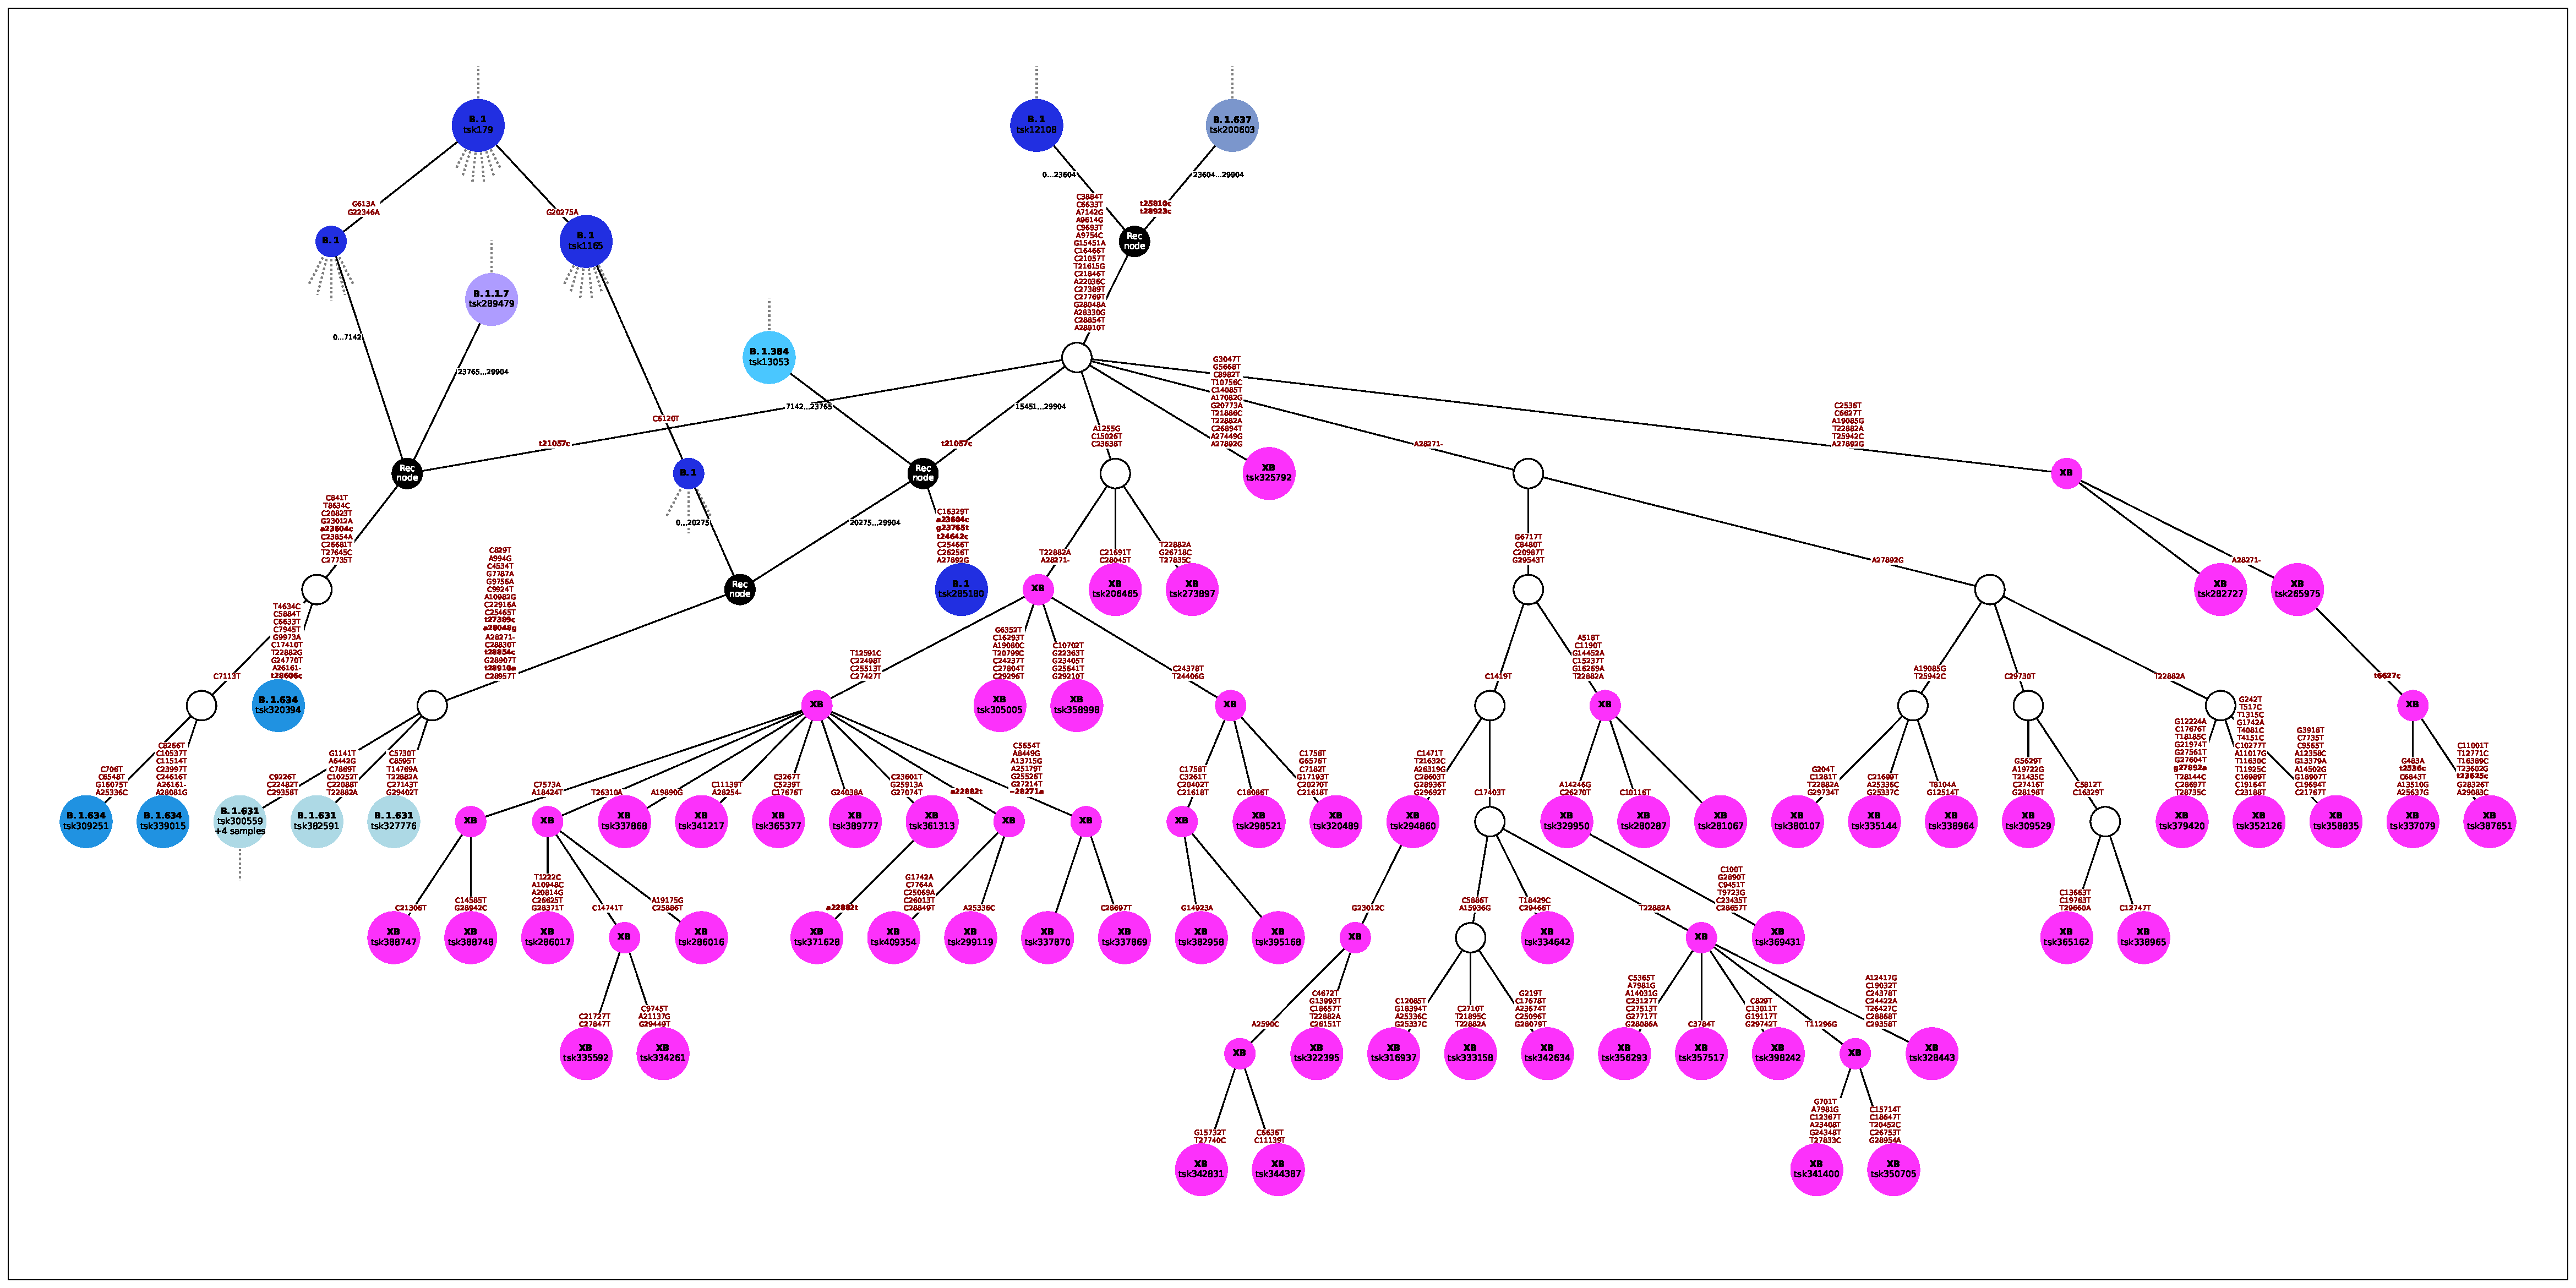
\includegraphics[width=\textwidth]{figures/Pango_XB_gisaid_large_graph.pdf}
\caption{\label{fig:pango_XB_gisaid_graph}  DESCRIBE ME}
\end{figure}

\end{document}
